\section{Introduction}
\begin{figure*}[h]
	\centering
	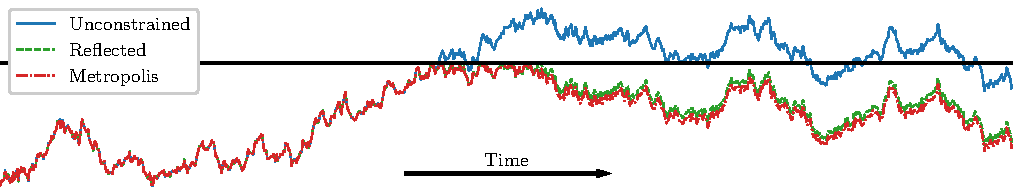
\includegraphics[width=\textwidth]{images/constraind_diffusion_rejection/rejection_vs_brownian_1d.pdf}

	\caption{Visual comparison of a discretisation of the unconstrained Brownian
		motion, two discretisations of the reflected Brownian motion: one based on
		a reflection scheme and the other based on our Metropolis sampler.
		The Metropolised trajectory is very close to that of the reflected one, while being significantly easier to implement and cheaper to compute.
	}
	\label{fig:1d_trajectories}
\end{figure*}

\lettrine{I}{n the previous chapter} we extended the applicability of diffusion models to inequality-constrained manifolds by investigating the generative modelling applications of classic sampling schemes based on log-barrier methods \parencite{Kannan2009,lee2017Geodesic,noble2022Barrier,kook2022sampling,gatmiry2022convergence,lee2018convergence} and the reflected Brownian motion \parencite{williams1987Reflected,petit1997Time,shkolnikov2013Timereversal}.
While empirically promising, the proposed algorithms can be computationally and numerically burdensome, and require bespoke implementations for different manifolds and constraints.

In this chapter, we propose a new method for generative modelling on constrained manifolds based on a Metropolis discretisation of the reflected Brownian motion.
This Metropolised discretisation has two main advantages:
\begin{enumerate}
	\item From a technical perspective it is lightweight: the only additional requirement over those outlined in \cref{cpt:riemannian_score_based_models} that is needed to implement a constrained diffusion model is a binary function that indicates whether any given point is within the constrained set. This is in contrast to the methods of \cref{cpt:constrained_domains} which require significantly more components.
	\item From a computational perspective it is much cheaper to compute, and more numerically stable than the methods proposed in  \cref{cpt:constrained_domains}.
\end{enumerate}
Our core theoretical contribution is to show that this new discretisation converges to the reflected stochastic differential equation by using the invariance principle for stochastic differential equations with boundary \parencite{stroock1971diffusion}.

To the best of our knowledge, this is the first time that such a process has been investigated in a machine learning context, or elsewhere.
We demonstrate that our method attains improved empirical results on manifolds with convex and non-convex constraints by applying it to a range of problems from geospatial modelling, robotics and protein design.

\section{Diffusion models for constrained manifolds via Metropolis sampling}
\label{sec:methodology}

In~\cref{sec:practical_constraints}, we highlight the practical limitations of existing constrained diffusion models in \cref{sec:metropolis_scheme} propose an alternative Metropolis sampling-based approach.
In \cref{sec:theoretical_convergence}, we outline our proof that this process corresponds to a valid discretisation of the reflected Brownian motion, justifying its use in diffusion models.
An overview of the samplers, and the various operations required to run them, we cover in this section are presented in~\cref{tab:general_method_comparison}.
\Cref{tab:general_method_comparison2} compares the computational cost of training various instantiations of constrained diffusion models, and the geometric domains they cover.

The technical setting we consider in this chapter is the same as in \cref{cpt:constrained_domains}.
Briefly, given a Riemannian manifold \((\c{N}, {h})\), we consider a family of real functions \(\{f_i: \c{N} \to \R\}_{i \in \mathcal{I}}\) indexed by \(\mathcal{I}\).
We then define \begin{equation} \label{eq:constrained} \c{M} = \cbr{x \in \c{N} \; : \; f_i(x) < 0 , \ i \in \mathcal{I}},
\end{equation}
and derive models such that their densities are constrained to be in the set \(\c{M}\).
A more detailed description of the setting can be found in \cref{sec:constrained_diffusion_models}.

\subsection{Practical limitations of existing constrained diffusion models}
\label{sec:practical_constraints}

\begin{figure}[t]
	\centering
	\begin{subfigure}[t]{0.48\textwidth}
		\centering
		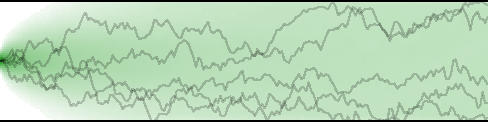
\includegraphics[width=\textwidth]{images/constraind_diffusion_rejection/reflected_density_no_text.pdf}
		\caption{Reflected Brownian motion}
	\end{subfigure}
	\hfill
	\begin{subfigure}[t]{0.48\textwidth}
		\centering
		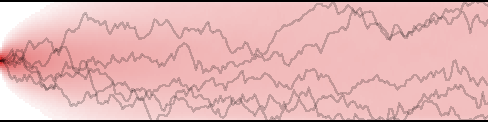
\includegraphics[width=\textwidth]{images/constraind_diffusion_rejection/rejection_density_no_text.pdf}
		\caption{Metropolised approximation of Brownian motion}
	\end{subfigure}
	\caption{Evolution of the density of the reflected Brownian motion and its Metropolis sampling-based approximation on the unit interval starting from a delta mass.}
	\label{fig:1d_densities}
\end{figure}

\paragraph{Barrier metrics.}
In the barrier approach, \cref{sec:bsgm}, the constrained manifold is transformed into an unconstrained space via a barrier metric.
This metric is defined by \[g=\nabla^2 \phi(x),\quad \phi(x) = \sum_{i\in \c{I}} \phi(d(x, f_i)),\] where \(d(x, f_i)\) is the minimum distance from the point \(x\) to the set defined by \(f_i(x) = 0\) and \(\phi_i\) is a monotone decreasing function such that \(\lim_{z \rightarrow 0} \phi_i(z) = \infty\).
Under additional regularity assumptions, \(\phi\) is called a \emph{barrier function}, see \cite{nesterov1994interior}.
This metric replaces the original metric on the space, warping the geometry.
This definition ensures that the barrier function induces a well-defined exponential map on the manifold, making the Riemannian diffusion model framework \cref{cpt:riemannian_score_based_models} apply.

In practice, evaluating \(\phi\) requires computing \(d(x, \partial f_i)\) (and its derivatives), which can be prohibitively expensive.
Furthermore, since the exponential under the induced manifold is not easy to compute, in the barrier method it is approximated by projecting the exponential of the original metric back into the constrained set.
This incurs additional bias and necessitating a step projecting samples back inside the constraints, which can itself be computationally intractable, see \textcite{absil2012projection, boumal2023introduction}.

\emphmarginnote{Mirror diffusion models} \cite{tae2023mirror,liu2024mirror} work on similar principles to the barrier methods in \cref{sec:bsgm}.
Instead of modelling on the original space, they project the data space under the map \(\nabla \phi: \c{M} \to \R^d\).
For convex \(\c{M}\subset \R^d\) this is a bijection.
This allows for the placing of a diffusion model on Euclidean space and pulling it back onto the original constrained space, a procedure reminiscent of the baseline introduced in \cref{sec:stereo_exp}.
It suffers from the same issue as the barrier method, warping the underlying geometry of \(\c{M}\), but does enjoy faster training.

\paragraph{Reflected stochastic processes.}
The alternative approach explored in \cref{cpt:constrained_domains} is based on reflected Brownian motion.
One possible discretisation of the reflected SDE is to \begin{enumerate*}[label=(\roman*)] \item consider a classical step of the Euler-Maruyama discretisation (or the Geodesic Random Walk in the Riemannian setting) and \item reflect this step according to the boundary defined by \(\partial \c{M}\).
\end{enumerate*}
To compute the reflection, one must check whether the step crosses the boundary.
If it does, the point of intersection needs to be calculated, the ray reflected at this point, and the step continued in the reflected direction.
This can require an arbitrarily large number of reflections depending on the step size, the geodesic on the manifold, and the geometry of the bounded region within the manifold.
We refer to \cref{sec:rbm} and \cref{alg:reflection} for the detail of the typical reflection discretisation.

\textcite{lou2023reflected} also consider a reflected Brownian motion for diffusion modelling.
By considering a restricted setting of the hypercube they obtain an analytic form of sampling for the forward noising process and denoising score matching.
However, to model more complex constraints they require a step to warp the constraints into the hypercube, modifying the geometry of the problem.

An alternative approach to discretising a reflected stochastic differential equation is to replace the reflection with a projection, see \cite{slominski1994approximation} for instance.
However, the projection still requires the most expensive part of the reflection algorithm: computing the intersection of the geodesic with the boundary.

\subsection{Metropolis approximation of reflected Brownian motion}
\label{sec:metropolis_scheme}
As outlined in the previous section, both of the existing approaches for constrained diffusion models require manifold- and constraint-specific implementations, and become computationally intractable as the complexity and dimension of the modelled geometry increases.

This limits their practical usefulness even for relatively simple manifolds with well-defined exponential maps and linear inequality constraints (such as e.g. polytopes).

In \cref{alg:metropolis_approx} we introduce a method that aims to solve both of these problems.
\begin{algorithm}[H]
	\caption[]{\protect\marginnote{Metropolis approximation of reflected Brownian motion step}}
	\label{alg:metropolis_approx}
	\begin{algorithmic}
		\Require \(p \in \c{M}\), \(\{f_i\}_{i \in \c{I}}\)
		\State Sample \(\v{v} \sim \mathrm{N}(0,\m{I}) \in \mathrm{T}_p\c{M}\)
		\State \(p' \gets \exp_{p}(\v{v})\)
		\If{\(f_i(p') < 0\ \forall\ i\)}
		\State \(p\gets p'\)
		\EndIf
		\Return \(p\)
	\end{algorithmic}
\end{algorithm}
The discretisation step sampler we propose is similar to a classical Euler-Maruyama discretisation of the Brownian motion, except that, whenever a step would carry the Brownian motion outside the constrained region, we reject it.
This is a \emph{Metropolised} version of the usual discretisation and is almost trivial to implement compared to the existing barrier, reflection, and projection methods.
Hence, this method enables the principled extension of diffusion models to arbitrarily constrained domains at virtually \emph{no added implementation complexity or computational expense}.

\begin{table*}[t]
	\centering
	\small
	\caption{Comparing the requirements of different constrained diffusion models. Distance to boundary and intersection operations are typically significantly more expensive to compute, and in some setting intractable. Set indicator functions are typically more lightweight and more commonly available on any given domain. Methods that rely on set indicator functions only are therefore computationally efficient.}
	\label{tab:general_method_comparison}

	\begin{tabular}{lccc}
		\toprule
		\thead[l]{\scshape Sampling Method}                                  & \thead[c]{\scshape Set Indicator \\\scshape Function} & \thead[c]{\scshape Intersection\\\scshape Operator} & \thead[c]{\scshape Distance to\\\scshape Boundary} \\
		\midrule
		\scshape Barrier method (\Cref{cpt:constrained_domains})             & \cmark                  & \cmark & \cmark \\
		\scshape Mirror diffusion \parencite{liu2024mirror}	 & \cmark                  & \cmark & \cmark \\
		\scshape Reflected method (\Cref{cpt:constrained_domains}, \textcite{lou2023reflected}) & \cmark                  & \cmark & \xmark \\
		\scshape Projection sampler \parencite{lou2023reflected}             & \cmark                  & \cmark & \xmark \\
		\scshape Metropolis sampler (This chapter)                                   & \cmark                  & \xmark & \xmark \\
		\bottomrule
	\end{tabular}
\end{table*}

\begin{table*}[t]
	\centering
	\small
	\caption{Comparison of the advantages and disadvantages of the different constrained (Riemannian) diffusion models covered in~\Cref{sec:practical_constraints} with regard to training the score function and preserving the geometry of the domain. The methods proposed in \cref{cpt:constrained_domains} and this chapter can be applied to arbitrary manifolds while preserving the underlying geometry of the manifold. However, this comes at the cost of making denoising score matching intractable and falling back on implicit score matching. By contrast the methods of \textcite{lou2023reflected,liu2024mirror} allow for the use of denoising score matching, but are limited to being applied ot Euclidean space, or warping the underlying geometry of a space. It should be noted that if the reflected method of \cref{cpt:constrained_domains} is applied to the same setting as \textcite{lou2023reflected} then we can make use of denoising score matching in the same way.}
	\label{tab:general_method_comparison2}
	\vspace{1em}
	\begin{tabular}{lcccc}
		& \multicolumn{2}{c}{\(\overbracket{\mspace{200mu}}^{\text{\small Both required for fast DSM loss}}\)} &  & \\
		\toprule
		\scshape \bfseries Diffusion Model & \scshape \thead[c]{Tractable \\conditional score} & \scshape \thead[c]{Simulation-free\\forward sampling} & \scshape \thead[c]{Modelling                            \\domain}  & \scshape \thead[c]{Preserves\\metric of \(\c{M}\)} \\
		\midrule
		\scshape Reflected Diffusions                                                                                               \\
		\quad\scshape \textcite{lou2023reflected}         & \cmark                    & \cmark & \(\text{\small convex}\;{\subset}\;\mathbb{R}^d\)       & \xmark \\
		\quad\scshape \cref{cpt:constrained_domains}  & \xmark                    & \color{black!50!red}\(\c{O}(d^2)\) & \(\text{\small convex}\;{\subset}\;\text{any}\;\c{M}\)           & \cmark \\
		\quad\scshape This chapter & \xmark                    & \color{black!50!red}\(\c{O}(d)\) & \(\text{\small convex}\;{\subset}\;\text{any}\;\c{M}\)             & \cmark \\

		\midrule
		\scshape Barrier Diffusions                                                                                                 \\
		\quad\scshape \cref{cpt:constrained_domains}  & \xmark                    & \xmark \hspace{0.1em} & \(\text{\small convex}\;{\subset}\;\text{any}\;\c{M}\)             & \xmark \\
		\quad\scshape \textcite{liu2024mirror}            & \cmark                    & \cmark & \(\text{\small convex}\;{\subset}\;\mathbb{R}^d\) & \xmark \\

		\bottomrule
	\end{tabular}
\end{table*}

\subsection{Convergence of the Metropolis sampler to the reflected Brownian motion}
\label{sec:theoretical_convergence}

In this section, we prove that the proposed Metropolis sampling-based process (\cref{alg:metropolis_approx}) corresponds to a valid discretisation of the reflected process, \cref{eq:rbm}, justifying its use in diffusion models.
Here we focus on a concise presentation of the core concepts and the main results.
A full proof can be found in \cref{sec:rejection-convergence}.

\subsubsection{Technical setting of the result}

For simplicity, we restrict ourselves to the Euclidean setting with smooth convex boundaries.
More specifically, for a function \(\Phi: \R^n \to \R\) defining the constrained set, \(\c{M} = \cbrcolon{x \in \R^d}{\Phi(x) > 0}\), we assume that this set is bounded and that \(\Phi \in \c{C}^2(\R^d, \R)\) concave.
In addition, we assume that for any \(x \in \partial \c{M}\), \(\norm{\nabla \Phi(x)} = 1\).
These assumptions match those \textcite{stroock1971diffusion} use for their study of the existence of solutions to the reflected Brownian motion.

While it seems possible to relax the \emph{global} existence of \(\Phi\) to a \emph{local} one, i.e. local concavity, the global regularity assumption of the domain, \(\Phi \in \c{C}^2(\R^d, \R)\), is key.
This regularity is essential to establish \cref{lemma:lower_bound_prob_main} and the associated geometrical result on tubular neighbourhoods.
The smoothness of the domain boundary is central in the results of \textcite{kang2017submartingale} on the equivalence of two definitions of reflected Brownian motion which we rely on.
As in \cref{cpt:constrained_domains}, we note it is possibly to infinitesimally smooth non-smooth boundaries to match the technical setting with very minimal practical impact.

It also seems possible to extend these results to the more general manifold setting, but this is technically challenging and outside the scope of this work.

In \cref{sec:exp_wildfires} we show however that the proposed algorithm does appear to practically work on a non-Euclidean manifold with non-convex, non-smooth boundaries.

\subsubsection{High level proof}
We begin with a definition of the Metropolis approximation of reflected Brownian motion.

\begin{definition}[Metropolis approximation of reflected Brownian motion]
	For any \(\gamma >0\) and \(k \in \N\), let \(X_0^\gamma \in \c{M}\) and 
	\[
		X_{k+1}^\gamma = \left\{ \begin{array}{lll}
			X_k^\gamma + \sqrt{\gamma} Z_k^\gamma & \text{ if } & X_k^\gamma + \sqrt{\gamma} Z_k^\gamma \in \c{M} \\
			X_k^\gamma & \text{ else } &
		\end{array} \right. .
	\]
	For \(Z_k \sim \c{N}(0, I)\).
	The sequence \((X_k^\gamma)_{k \in \N}\) is called the \emph{Metropolis approximation of reflected Brownian motion}.
\end{definition}
For any \(\gamma > 0\), we consider \((\v{X}_t^\gamma)_{t \geq 0}\), the linear interpolation of \((X^\gamma_k)_{k \in \N}\) such that for any \(k \in \N\), \(\v{X}_{k \gamma}^\gamma = X_k^\gamma\).
The following result is the main theoretical contribution of this section.

\begin{theorem}[Convergence of the Metropolis approximation to the reflected Brownian motion]
	\label{thm:weak_convergence_metropolis}
	Under assumptions on \(\c{M}\), for any \(T \geq 0\), \((\v{X}_t^\gamma)_{t \in \cbr{0,T}}\) weakly converges to the reflected Brownian motion \((\bar{\v{B}}_t)_{t \in \cbr{0,T}}\) as \(\gamma \to 0\).
\end{theorem}

The rest of the section is devoted to a high level presentation of the proof of \cref{thm:weak_convergence_metropolis}.

It is theoretically impractical to work directly with the Metropolis approximation of reflected Brownian motion.
Instead, we introduce an auxiliary process, show this converges to the reflected Brownian motion, and finally prove that the convergence of the auxiliary process implies the convergence of our Metropolis discretisation.
We define this auxiliary process now.

\begin{definition}[Rejection approximation of reflected Brownian motion]
	For any \(\gamma > 0\) and \(k \in \N\), let \(\hat{X}_0^\gamma \in \c{M}\) and \(\hat{X}_{k+1}^\gamma = \hat{X}_k^\gamma + \sqrt{\gamma} Z_k^\gamma\) with \(Z_k^\gamma\) a Gaussian random variable conditioned on \(\hat{X}_k^\gamma + \sqrt{\gamma} Z_k^\gamma \in \c{M}\).
	The sequence \((\hat{X}_k^\gamma)_{k \in \N}\) is called the \emph{rejection approximation of reflected Brownian motion}.
\end{definition}
We call this process the \emph{rejection approximation of reflected Brownian motion} since in practice, \(Z_k^\gamma\) can be sampled using rejection sampling, see~\cref{alg:rejection_sampling}.
\begin{algorithm}[H]
	\caption[]{\protect\marginnote{Rejection approximation of reflected Brownian motion}}
	\label{alg:rejection_sampling}
	\begin{algorithmic}
		\Require \(p \in \c{M}\), \(\{f_i\}_{i \in \c{I}}\)
		\State Sample \(\v{v} \sim \mathrm{N}(0,\m{I}) \in \mathrm{T}_p\c{M}\)
		\State \(p' \gets \exp_{p}(\v{v})\)
		\While{\(f_i(p') \geq 0\ \text{for any}\ i\)}
		\State Sample \(\v{v} \sim \mathrm{Id}(0,1) \in \mathrm{T}_p\c{M}\)
		\State \(p' \gets \exp_{p}(\v{v})\)
		\EndWhile
		\Return \(p'\)
	\end{algorithmic}
\end{algorithm}
The key difference between the rejection and Metropolis approaches is that where the Metropolis approach will leave the point stationary if the update falls outside the boundary, the rejection approach will resample the update until it lies inside the boundary.
This leaves the transition measures of these two processes the same, except the Metropolis version contains a Dirac component at the initial point.
While it is possible to implement the rejection approach practically, it is less desirable as it results in loops of unknown length in the sampling.

For any \(\gamma > 0\), we also consider \((\hat{\v{X}}_t^\gamma)_{t \geq 0}\), the linear interpolation of \((\hat{X}^\gamma_k)_{k \in \N}\) such that for any \(k \in \N\), \(\hat{\v{X}}_{k \gamma}^\gamma = \hat{X}_k^\gamma\).
In~\cref{sec:rejection-convergence}, we prove the following result.

\begin{theorem}[Convergence of the rejection approximation to the reflected Brownian motion]
	\label{thm:weak_convergence_rejection}
	Under assumptions on \(\c{M}\), for any \(T \geq 0\), \((\hat{\v{X}}_t^\gamma)_{t \in \cbr{0,T}}\) weakly converges to the reflected Brownian motion \((\bar{\v{B}}_t)_{t \in \cbr{0,T}}\) as \(\gamma \to 0\).
\end{theorem}

\begin{proof}
	For the full proof see \cref{sec:rejection-convergence}.
	Here we give some elements of the proof.

	Our approach is based on the invariance principle of \textcite{stroock1971diffusion}.
	More precisely, we show that we can compute an equivalent `drift' and `diffusion matrix' for the interpolated discretised process and that, as \(\gamma \to 0\), the drift converges to zero and the diffusion matrix converges to \(\m{I}\).

	In the Euclidean setting, this result, accompanied by mild regularity and growth assumptions, ensures that the discretisation weakly converges to the original stochastic differential equation.
	However, the case with boundary is much more complicated, primarily because the approximate drift might explode near the boundary, thus we need to verify exactly how the drift behaves as \(\gamma \to 0\) and as the process approaches the boundary.

	We show that the \emph{normalised} drift converges to the inward normal near the boundary.
	This ensures that \begin{enumerate}[label=(\alph*)] \item in the interior of \(\c{M}\) the drift converges to zero, i.e.~locally in the interior of \(\c{M}\) the Brownian motion and the reflected Brownian motion coincide, \item on the boundary, the drift pushes the samples inside the manifold according to the inward normal, mimicking \((\v{k}_t)_{t \geq 0}\) in \cref{eq:rbm}.
	\end{enumerate}
	Finally, with results from \textcite{stroock1971diffusion} and \textcite{kang2017submartingale}, we show the convergence to the reflected Brownian motion.
\end{proof}

Having established that the rejection process converges to the reflected Brownian motion, our next step is to show that the approximate drift and diffusion matrix of the Metropolised process are related to the approximate drift and diffusion terms of the rejection process via multiplication by the term 
\[
	\alpha^\gamma(x) = \P\sbr{x + \sqrt{\gamma} Z} \in \c{M}	
\]
for \(Z\sim \c{N}(0, \m{I})\).
Having established this, we can conclude the proof by noting that the approximate drift and the diffusion matrix in the rejection and Metropolis case coincide as \(\gamma \to 0\).
This is enough to apply the same results as in the rejection process, giving the desired convergence.

This requires the following result.
\begin{proposition}
	\label{lemma:lower_bound_prob_main}
	Under assumptions on \(\c{M}\), \(\forall \; \varepsilon > 0\), \(\exists \; \bar{\gamma} >0\) such that for any \(\gamma \in \del{0, \bar{\gamma}}\) and for any \(x \in \c{M}\), we have \(\mathbb{P}(x + \sqrt{\gamma} Z \in \c{M}) \geq 1/2-\varepsilon\), with \(Z \sim \mathrm{N}(0, \m{I})\).
\end{proposition}

\Cref{lemma:lower_bound_prob_main} tells us that \emph{locally} the boundary
looks like a half-space when integrating with respect to. a Gaussian measure.
The assumption on the smoothness of the boundary is key in proving this result.
A corollary is that, for \(\gamma > 0\) small enough and for any \(k \in \N\), the probability that \(X_{k+1}^\gamma = X_k^\gamma\) is upper bounded \emph{uniformly} with respect to.
\(X_k^\gamma \in \c{M}\).
The proof of \cref{lemma:lower_bound_prob_main} uses \cref{thm:tubul-neighb} whose proof relies on the concept of \emph{tubular neighbourhoods} \parencite{lee2013smooth}.

\section{Related work on approximations of reflected stochastic differential equations}

Several schemes have been introduced to approximately sample from reflected stochastic differential equations.
They can be interpreted as modifications of classical Euler-Maruyama schemes used to discretise stochastic differential equations without boundary.
One of the most common approaches is to use the Euler-Maruyama discretisation and project the solution onto the boundary if it escapes from the domain \(\c{M}\).
In this case, mean-square error rates of order \emph{almost} \(1/2\) have been proven under various conditions \parencite{liu1995discretization,chitashvili1981strong,pettersson1995approximations,slominski1994approximation}.
Concretely this means that \(\E[\| \bar{\v{B}}_{t} - X_{n}^{t/n}\|^2] = O(n^{-1+\varepsilon})\) with \(\varepsilon>0\) arbitrary small and where \((X_k^\gamma)_{k \in \N}\) is the projection scheme.

The rate \(1/2\) is tight \parencite{pacchiarotti1998numerical}.
It is possible to use the Euler-Peano method to get slight improvements for a mean-square error rate of order of \(1/2\), but this is impractical as it assumes that one can solve a (simplified) Skorokhod problem, which is usually intractable.

\textcite{liu1993numerical} introduced a \emph{penalised}
method which pushes the solution away from the boundary and shows a mean-square error
of order \(1/4\), see also \cite{pettersson1997penalization}.
Weak errors of order \(1\) have been obtained in \textcite{bossy2004symmetrized} and \textcite{gobet2001euler} by introducing a reflection component in the discretisation or using some local approximation of the domain to a half-space.
We refer to \textcite{pilipenko2014introduction} for an introduction to the discretisation of reflected SDEs.
Closer to our work, \textcite{burdzy2008discrete} consider three different methods to approximate reflected Brownian motions on general domains (two based on discrete methods and one based on killed diffusions).
Only qualitative results are provided.
To the best of our knowledge, no previous work in the probability literature has investigated the \emph{Metropolised} scheme we propose.

Our Metropolis scheme is also related to the ball walk \parencite{applegate1991sampling}, which replaces the Gaussian random variable with a uniform over the ball (or the Dikin ellipsoid).
\textcite{applegate1991sampling} and \textcite{lovasz2007geometry} have
studied the asymptotic convergence rate of the ball walk, but, to the best of our
knowledge, its limiting behaviour when the step size goes to zero has not been
investigated.

\section{Experimental results}

To demonstrate the practical utility and empirical performance of the proposed Metropolis diffusion models, we conduct a comprehensive evaluation on a range of synthetic and real-world tasks.

In~\cref{sec:exp_synthetic_tasks}, we assess the scalability of our method by applying it to synthetic distributions on hypercubes and simplices of increasing dimension, similar to \cref{subsec:synthetic_data}.
In~\cref{sec:exp_arms_and_backbones}, we extend the evaluation to real-world tasks on manifolds with convex constraints by applying our method to the robotics and protein design datasets presented in \cref{subsec:psd_matrices,subsec:protein_loops}.

In~\cref{sec:exp_wildfires}, we additionally demonstrate that our method extends to constrained manifolds with highly \emph{non-convex} boundaries---a setting that is intractable with existing approaches.
As we found---in line with \cref{cpt:efficient_constrained_domains}---that log-barrier diffusion models perform strictly worse than reflected approaches across all experimental settings, we focus on a more detailed comparison with the latter here and postpone additional empirical results to~\cref{sec:app_exp_barrier_results}.

The code required to run the experiments in this chapter can be found \url{https://github.com/oxcsml/score-sde/tree/metropolis}.
Details of the experimental set up can be found in \cref{sec:app_implementational_details}.

\subsection{Synthetic distributions on simple polytopes}
\label{sec:exp_synthetic_tasks}

\begin{table}
	\caption{
		Log-likelihood (\(\uparrow\)) of a held-out test set from a synthetic bimodal distribution over convex subsets of \(\R^d\) bounded by the hypercube \([-1,1]^d\) and unit simplex \(\Delta^d\).
		Means and standard deviations are computed over 3 different runs.
		Training time in hours is listed in parentheses.
	}
	\label{tab:synthetic_polytope_dupref}
	\centering

	\begin{tabular}{clll}
		\toprule
		\scshape Constraint & \(d\) & {\scshape Reflected \emph{(hours)}}    & {\scshape Metropolis \emph{(hours)}}              \\
		\midrule
		\multirow{3}{*}{\([-1,1]^d\)}
		           & 2     & \(2.25\pm{.01}\) \emph{(8.95)}  & \(\mathbf{2.32\pm{.05}}\) \emph{(0.72)}    \\
		           & 3     & \(3.77\pm{.13}\) \emph{(8.97)}  & \(\mathbf{4.15\pm{.15}}\) \emph{(0.71)}    \\
		           & 10    & \(7.42\pm{.77}\) \emph{(10.15)} & \(\mathbf{10.80 \pm{.34 }}\) \emph{(0.90)} \\
		\midrule
		\multirow{3}{*}{\(\Delta^d\)}
		           & 2     & \(1.01 \pm{.01}\) \emph{(9.17)} & \(\mathbf{1.06\pm{.02}}\) \emph{(0.82)}    \\
		           & 3     & \(2.64\pm{.01}\) \emph{(9.43)}  & \(\mathbf{3.23\pm{.17}}\)  \emph{(0.78)}   \\
		           & 10    & \(7.00\pm{.13}\) \emph{(10.53)} & \(\mathbf{7.81\pm{.20}}\) \emph{(0.97)}    \\
		\bottomrule
	\end{tabular}
\end{table}

\begin{figure}[t]
	\centering
	\begin{subfigure}[t]{.23\textwidth}
		\centering
		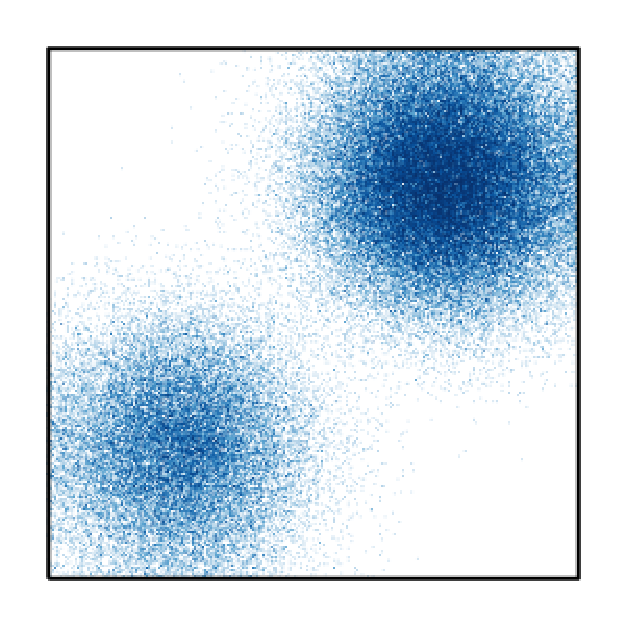
\includegraphics[width=\textwidth]{images/constraind_diffusion_rejection/synthetic_data/synthetic_hypercube_2d_data.pdf}
		\caption{Data distribution}
		\label{fig:app:synthetic_hypercube_data}
	\end{subfigure}
	\begin{subfigure}[t]{.23\textwidth}
		\centering
		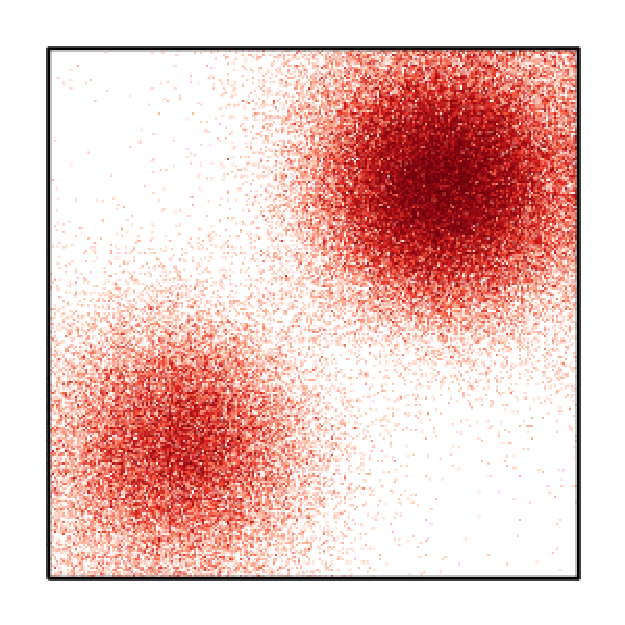
\includegraphics[width=\textwidth]{images/constraind_diffusion_rejection/synthetic_data/synthetic_hypercube_2d_rejection.pdf}
		\caption{Metropolis model}
		\label{fig:app:synthetic_hypercube_rejection}
	\end{subfigure}
	\begin{subfigure}[t]{.23\textwidth}
		\centering
		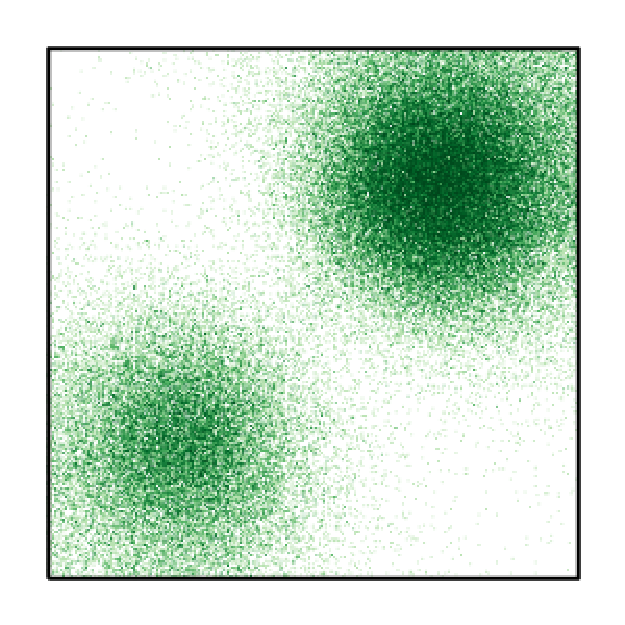
\includegraphics[width=\textwidth]{images/constraind_diffusion_rejection/synthetic_data/synthetic_hypercube_2d_reflected.pdf}
		\caption{Reflected model}
		\label{fig:app:synthetic_hypercube_reflected}
	\end{subfigure}
	\begin{subfigure}[t]{.23\textwidth}
		\centering
		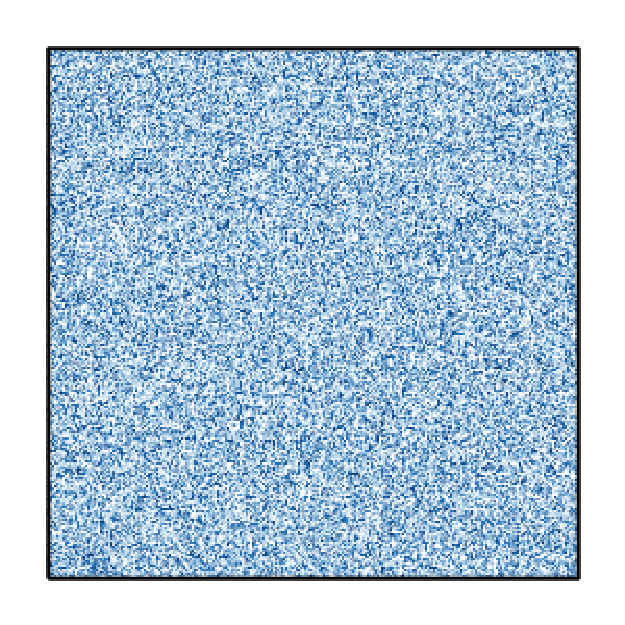
\includegraphics[width=\textwidth]{images/constraind_diffusion_rejection/synthetic_data/synthetic_hypercube_2d_uniform.pdf}
		\caption{Uniform distribution}
		\label{fig:app:synthetic_hypercube_uniform}
	\end{subfigure}
	\caption{Qualitative comparison of samples from the data distribution, our Metropolis model, a Reflected model and the uniform distribution for a synthetic bimodal distribution on $[-1, 1]^2$.}
	\label{fig:app:synthetic_hypercube}
\end{figure}

\begin{figure}[t]
	\centering
	\begin{subfigure}[t]{.23\textwidth}
		\centering
		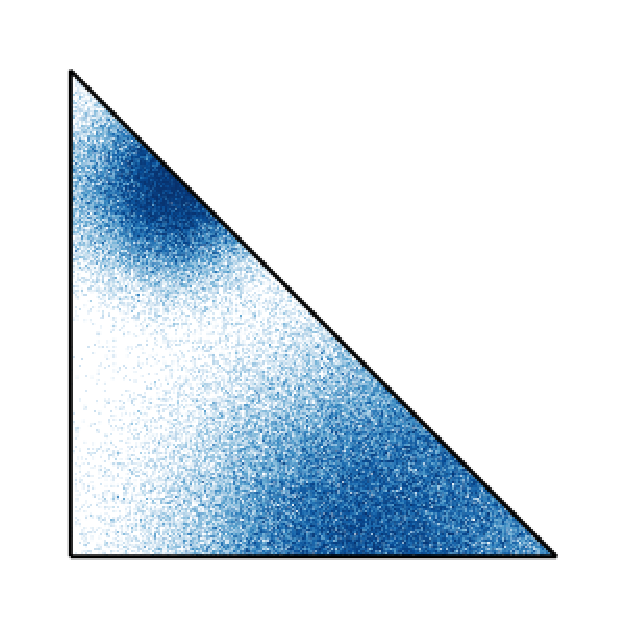
\includegraphics[width=\textwidth]{images/constraind_diffusion_rejection/synthetic_data/synthetic_dirichlet_2d_data.pdf}
		\caption{Data distribution}
		\label{fig:app:synthetic_simplex_data}
	\end{subfigure}
	\begin{subfigure}[t]{.23\textwidth}
		\centering
		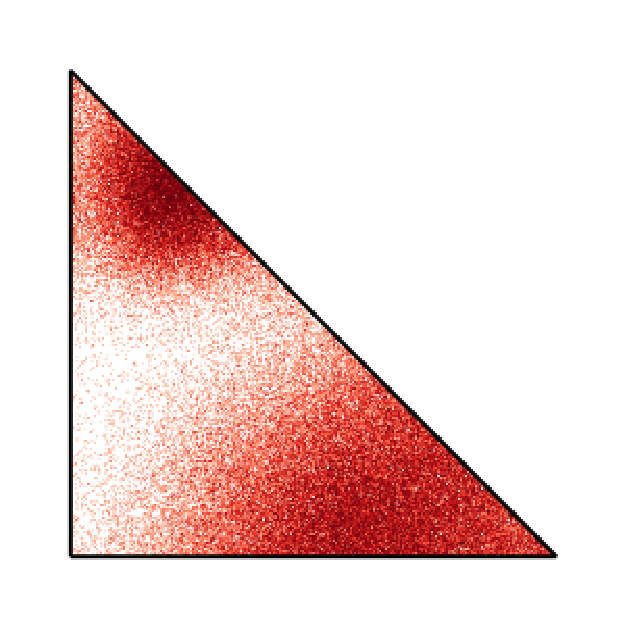
\includegraphics[width=\textwidth]{images/constraind_diffusion_rejection/synthetic_data/synthetic_dirichlet_2d_rejection.pdf}
		\caption{Metropolis model}
		\label{fig:app:synthetic_simplex_rejection}
	\end{subfigure}
	\begin{subfigure}[t]{.23\textwidth}
		\centering
		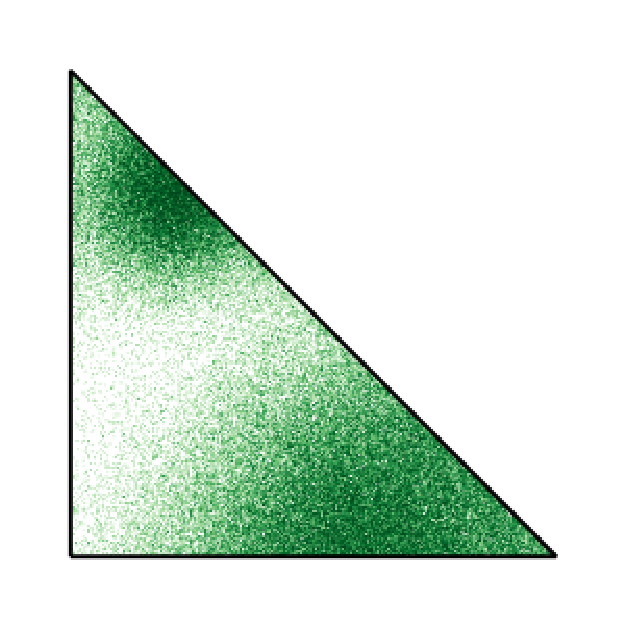
\includegraphics[width=\textwidth]{images/constraind_diffusion_rejection/synthetic_data/synthetic_dirichlet_2d_reflected.pdf}
		\caption{Reflected model}
		\label{fig:app:synthetic_simplex_reflected}
	\end{subfigure}
	\begin{subfigure}[t]{.23\textwidth}
		\centering
		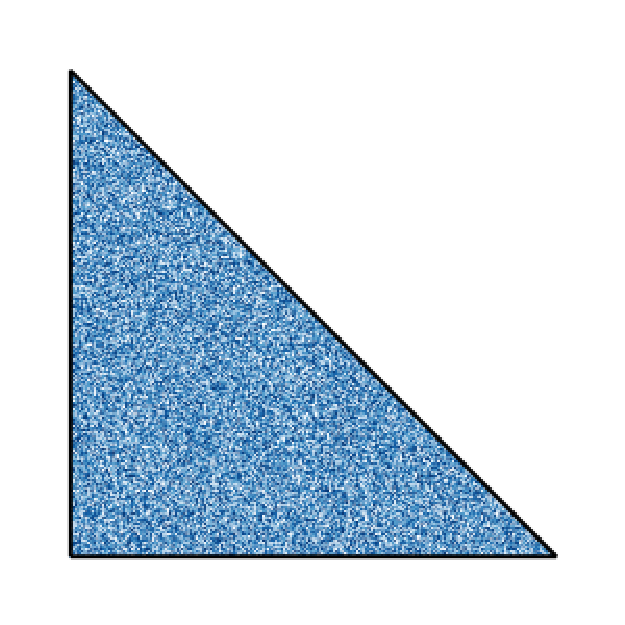
\includegraphics[width=\textwidth]{images/constraind_diffusion_rejection/synthetic_data/synthetic_dirichlet_2d_uniform.pdf}
		\caption{Uniform distribution}
		\label{fig:app:synthetic_simplex_uniform}
	\end{subfigure}
	\caption{Qualitative comparison of samples from the data distribution, our Metropolis model, a Reflected model and the uniform distribution for a synthetic bimodal distribution on $\Delta^2$.}
	\label{fig:app:synthetic_simplex}
\end{figure}

\begin{figure}
    \centering
    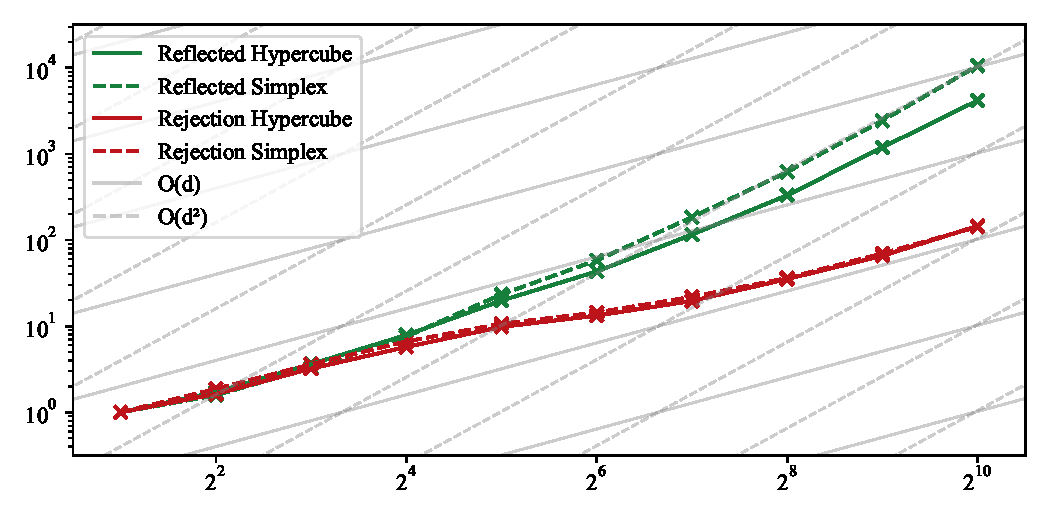
\includegraphics[width=0.9\textwidth]{images/constraind_diffusion_rejection/scaling.pdf}
    \put(-335, 20){\rotatebox{90}{\small Convergence time rel. to \(d=1\)}}
    \put(-210, 0){\small Dimension of manifold}
    \caption{Convergence time of the Reflected \textcolor{black!60!green}{(green)} and Metropolis \textcolor{black!60!red}{(red)} forward noising processes to the uniform distribution on the hypercube \([-1,1]^d\) and unit simplex \(\Delta^d\). The lines indicate functions fit with the \textsc{PySR} symbolic regression package \cite{cranmer2023interpretable} and correspond to empirical runtime complexities of \(\mathcal{O}(d^2)\) and \(\mathcal{O}(d)\), respectively, matching the superimposed scaling law isocontours.
    %\textcolor{gray}{(grey)}.
    }
    \label{fig:forward_process_timing}
\end{figure}

In this section, we investigate the scalability of the proposed Metropolis diffusion models by applying them to synthetic bimodal distributions over the \(d\)-dimensional hypercube \([-1, 1]^d\) and unit simplex \(\Delta^{d}\).
A quantitative comparison of the log-likelihood of a held-out test set is presented in~\cref{tab:synthetic_polytope_dupref}, while visual comparisons of the fitted distributions are shown in \cref{fig:app:synthetic_hypercube,fig:app:synthetic_simplex}.

We find that our Metropolis models outperform reflected approaches across all dimensions and constraint geometries by a substantial and statistically significant margin while training in one tenth of the time.

The degree of improvement seems to scale with the dimension of the problem; the larger the dimension of the experiment, the larger the gain in performance from using our proposed Metropolis scheme.

We observe a similar difference in the scaling properties of reflected and Metropolis models when measuring the convergence times of the respective forward noising processes to the uniform distribution on hypercubes \([-1, 1]^d\) and simplices \(\Delta^{d}\) of increasing dimension. The results are presented in~\cref{fig:forward_process_timing} and show that the convergence time of the Metropolis process scales linearly in the dimension, while the reflected process scales quadratically.

\subsection{Modelling proteins and robotic arms under convex constraints}
\label{sec:exp_arms_and_backbones}

In addition to illustrating our method's scalability on high-dimensional synthetic tasks, we follow the experimental setup from  \cref{subsec:psd_matrices,subsec:protein_loops} to demonstrate its practical utility and favourable empirical performance on two real-world problems from robotics and protein design.
We follow an identical problem set up, data, and model hyperparameters.

We quantify the empirical performance of different methods by evaluating the log-likelihood of a held-out test set and present the resulting performance metrics in~\cref{tab:real_world_data}.

Again, we find that our Metropolis model outperforms the reflected approach by a statistically significant margin while training 7-8 times as fast.
Qualitative visual comparisons of samples from the true distribution, the trained diffusion models and the uniform distribution are presented in~\cref{fig:robotic_arm,fig:loop}, with full univariate marginal and pairwise bivariate correlation plots postponed to~\cref{sec:app_robotic_arms_spd,sec:app_loop_pairplots}.

\begin{figure}[t]
	\centering
	\begin{subfigure}[t]{0.23\textwidth}
		\centering
		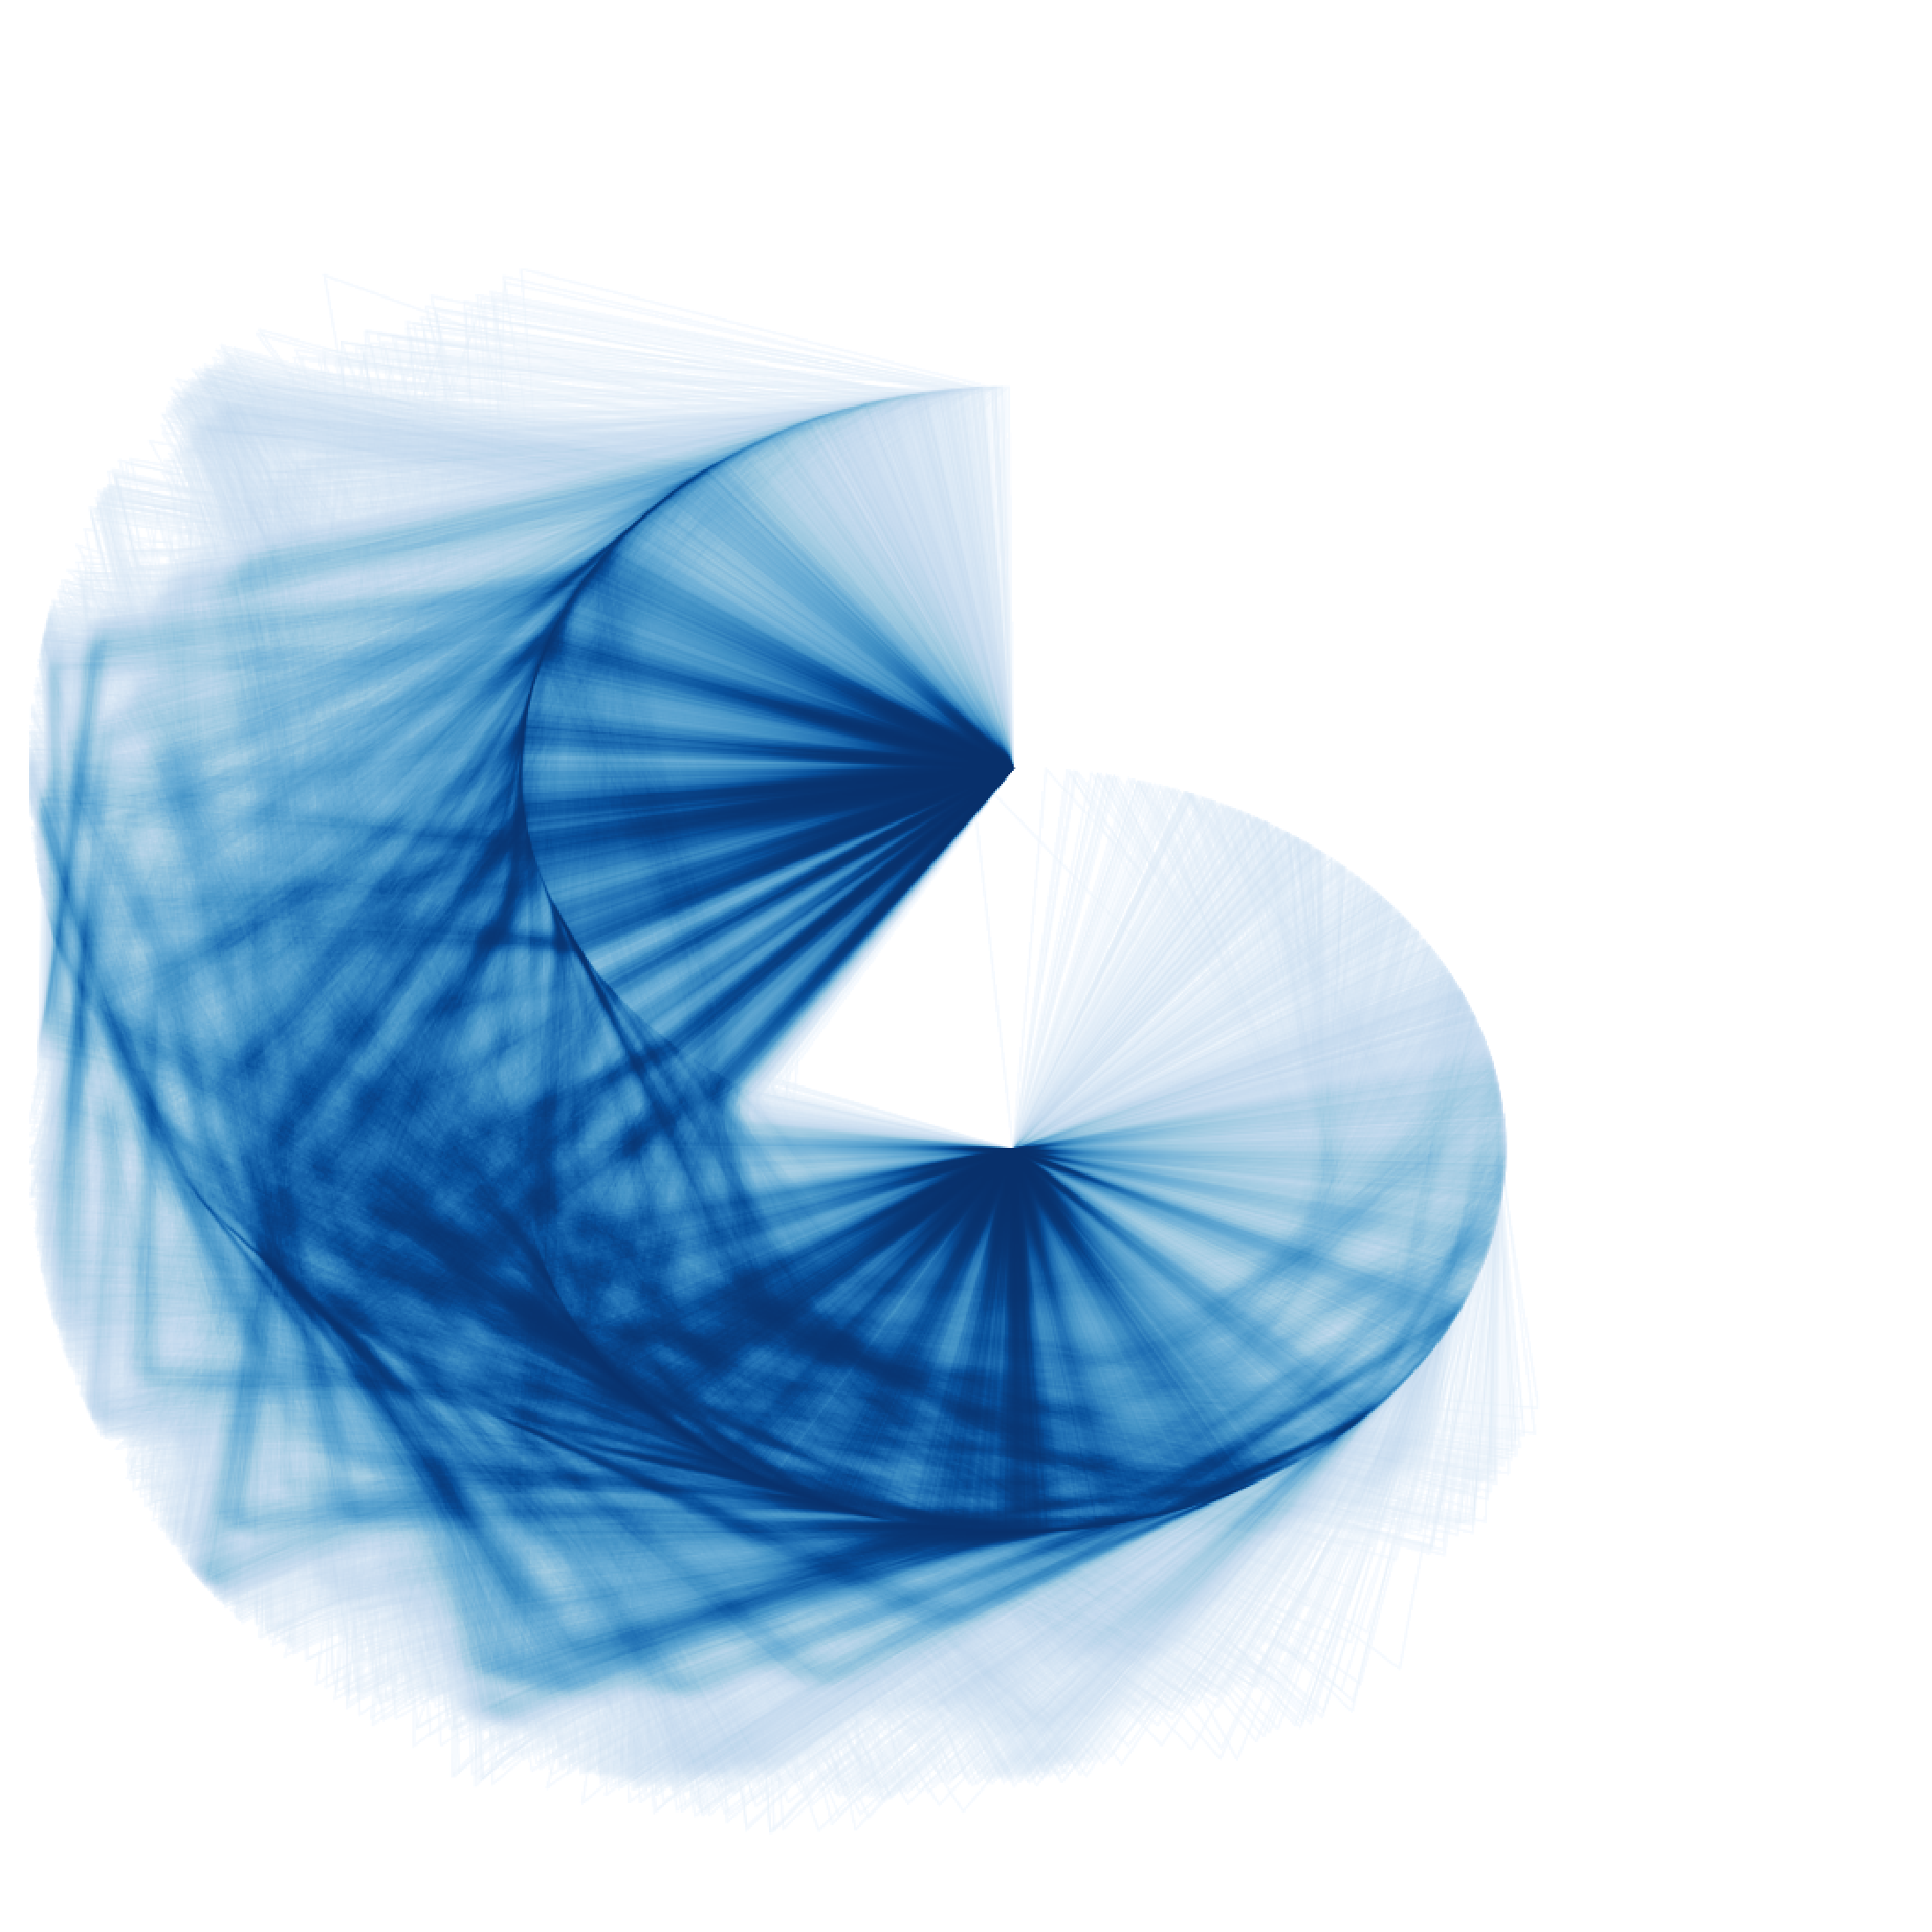
\includegraphics[width=\linewidth]{images/constraind_diffusion_rejection/loops_planar_data.pdf}
		\caption{Data distribution.}
		\label{fig:loop_data}
	\end{subfigure}
	\hfill
	\begin{subfigure}[t]{0.23\textwidth}
		\centering
		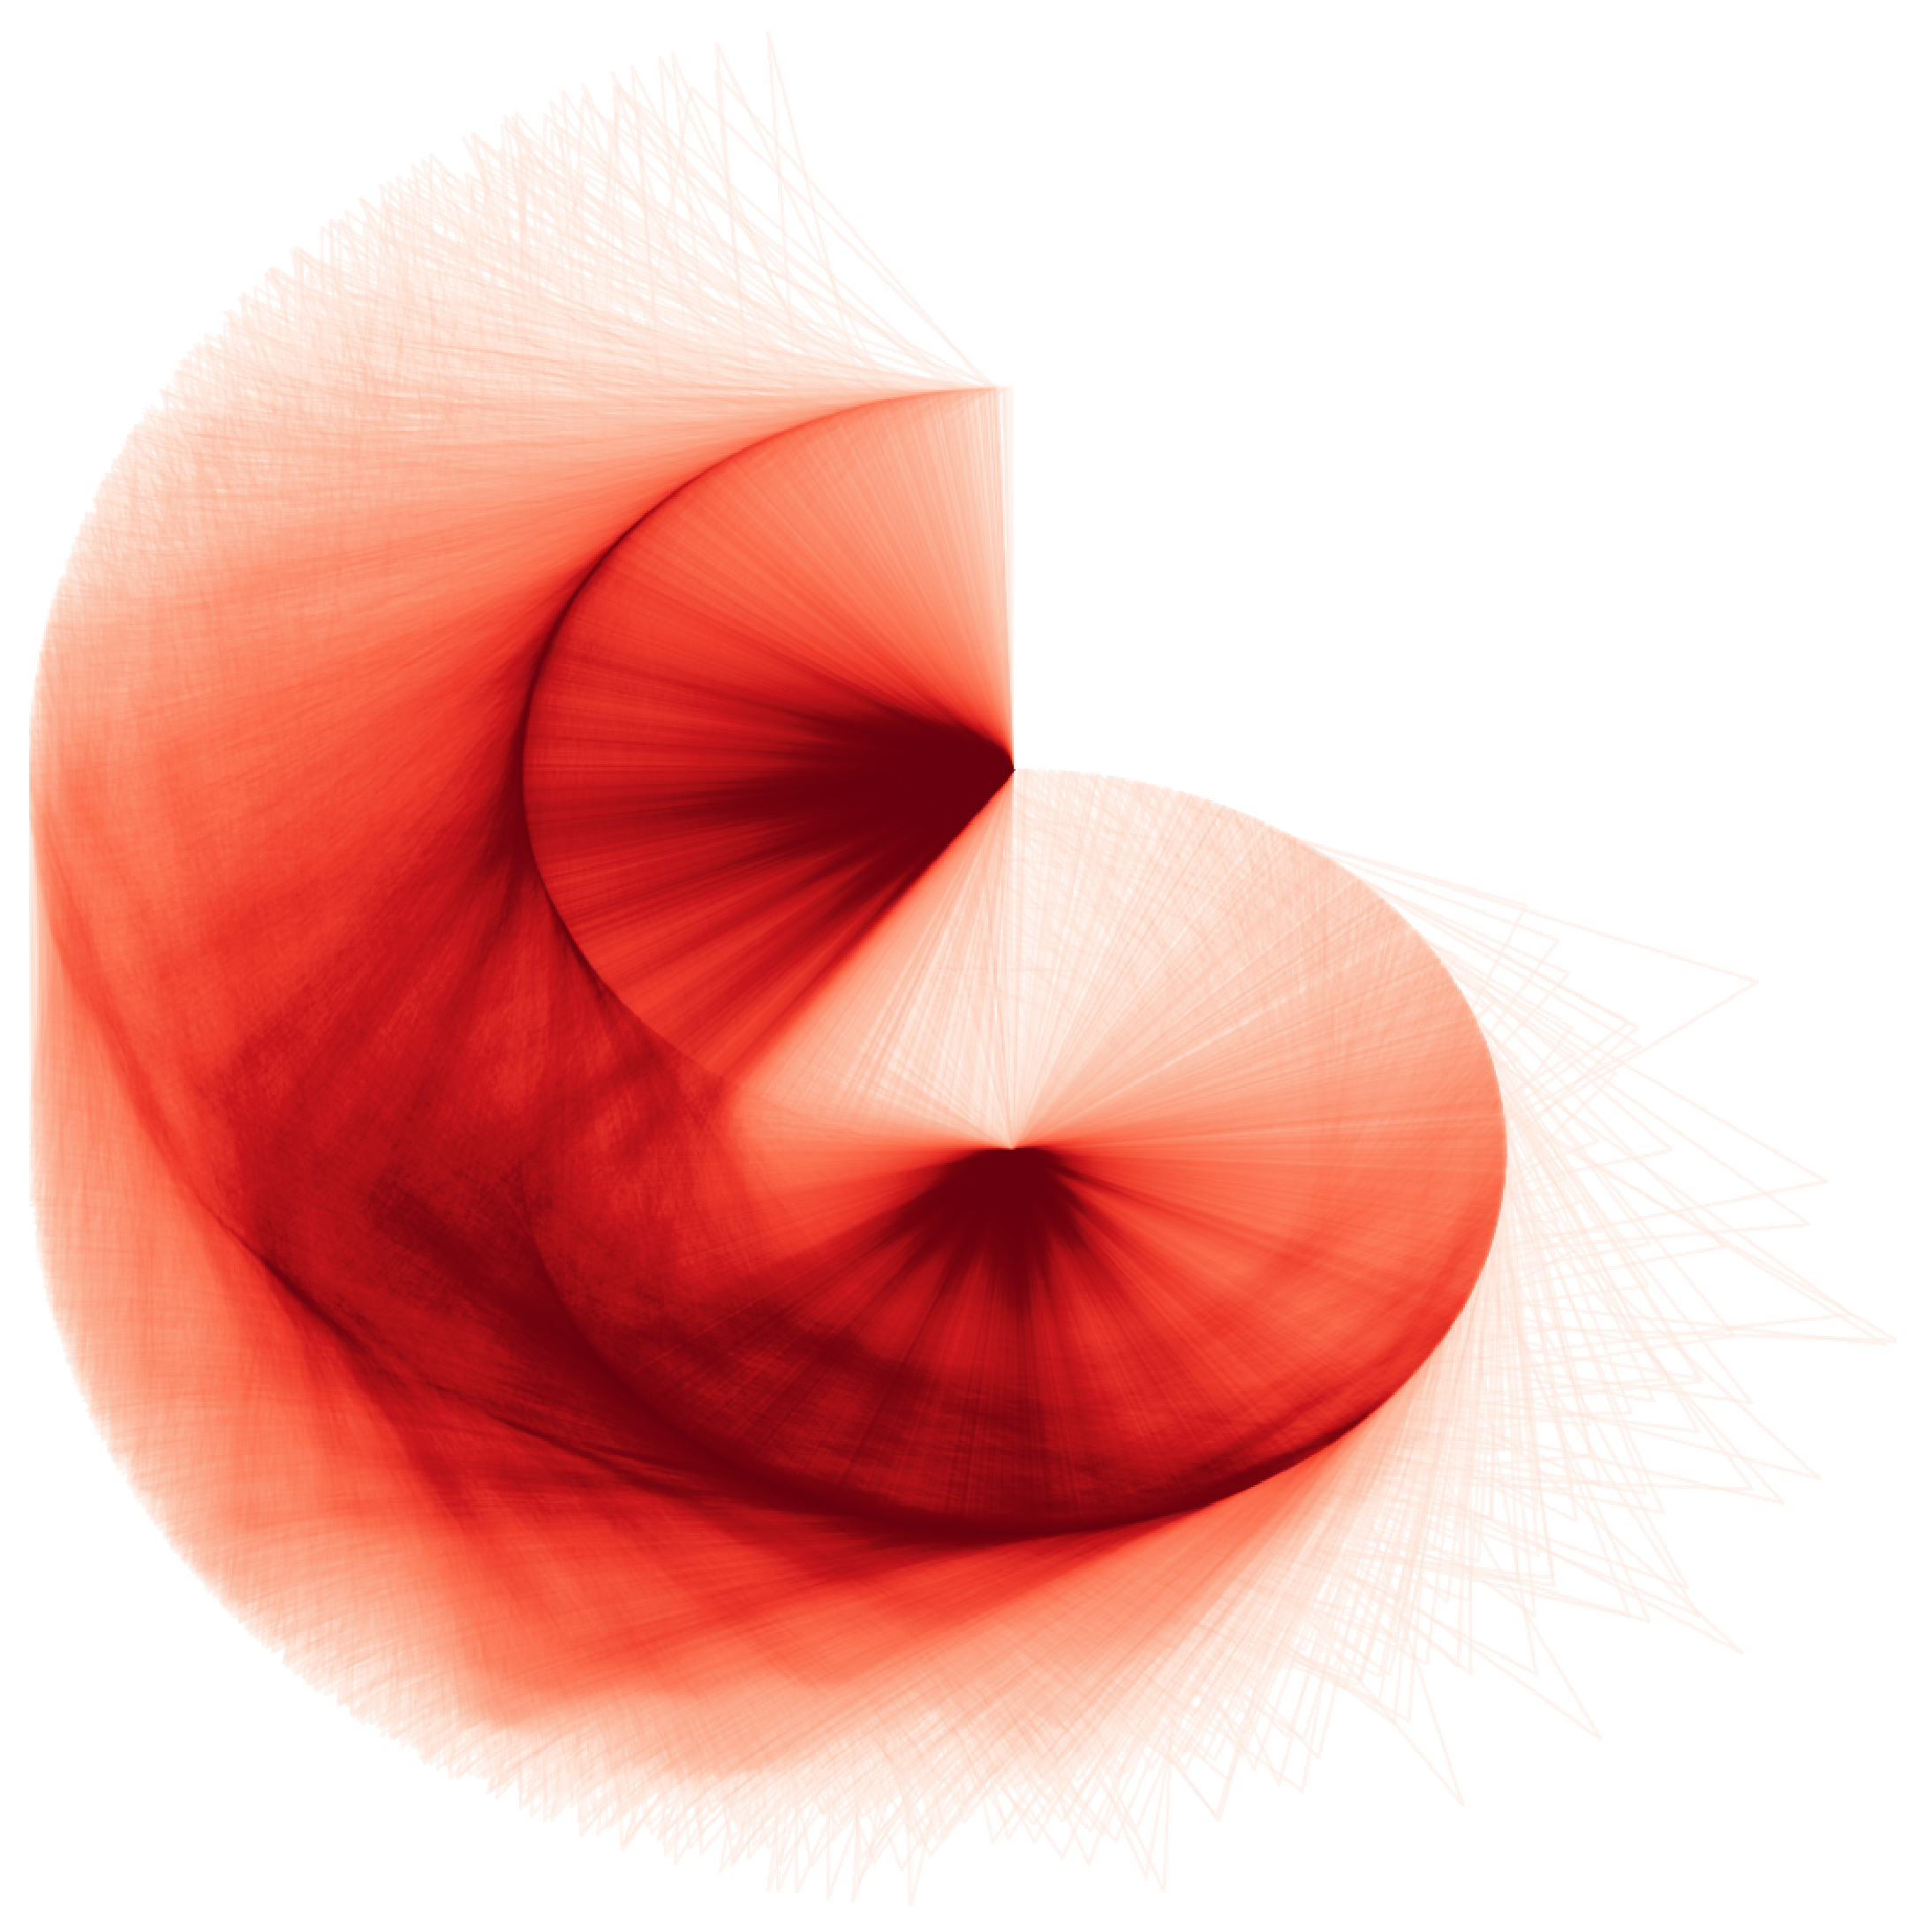
\includegraphics[width=\linewidth]{images/constraind_diffusion_rejection/loops_planar_rejection.pdf}
		\caption{Metropolis samples.}
		\label{fig:loop_rejection}
	\end{subfigure}
	\hfill
	\begin{subfigure}[t]{0.23\textwidth}
		\centering
		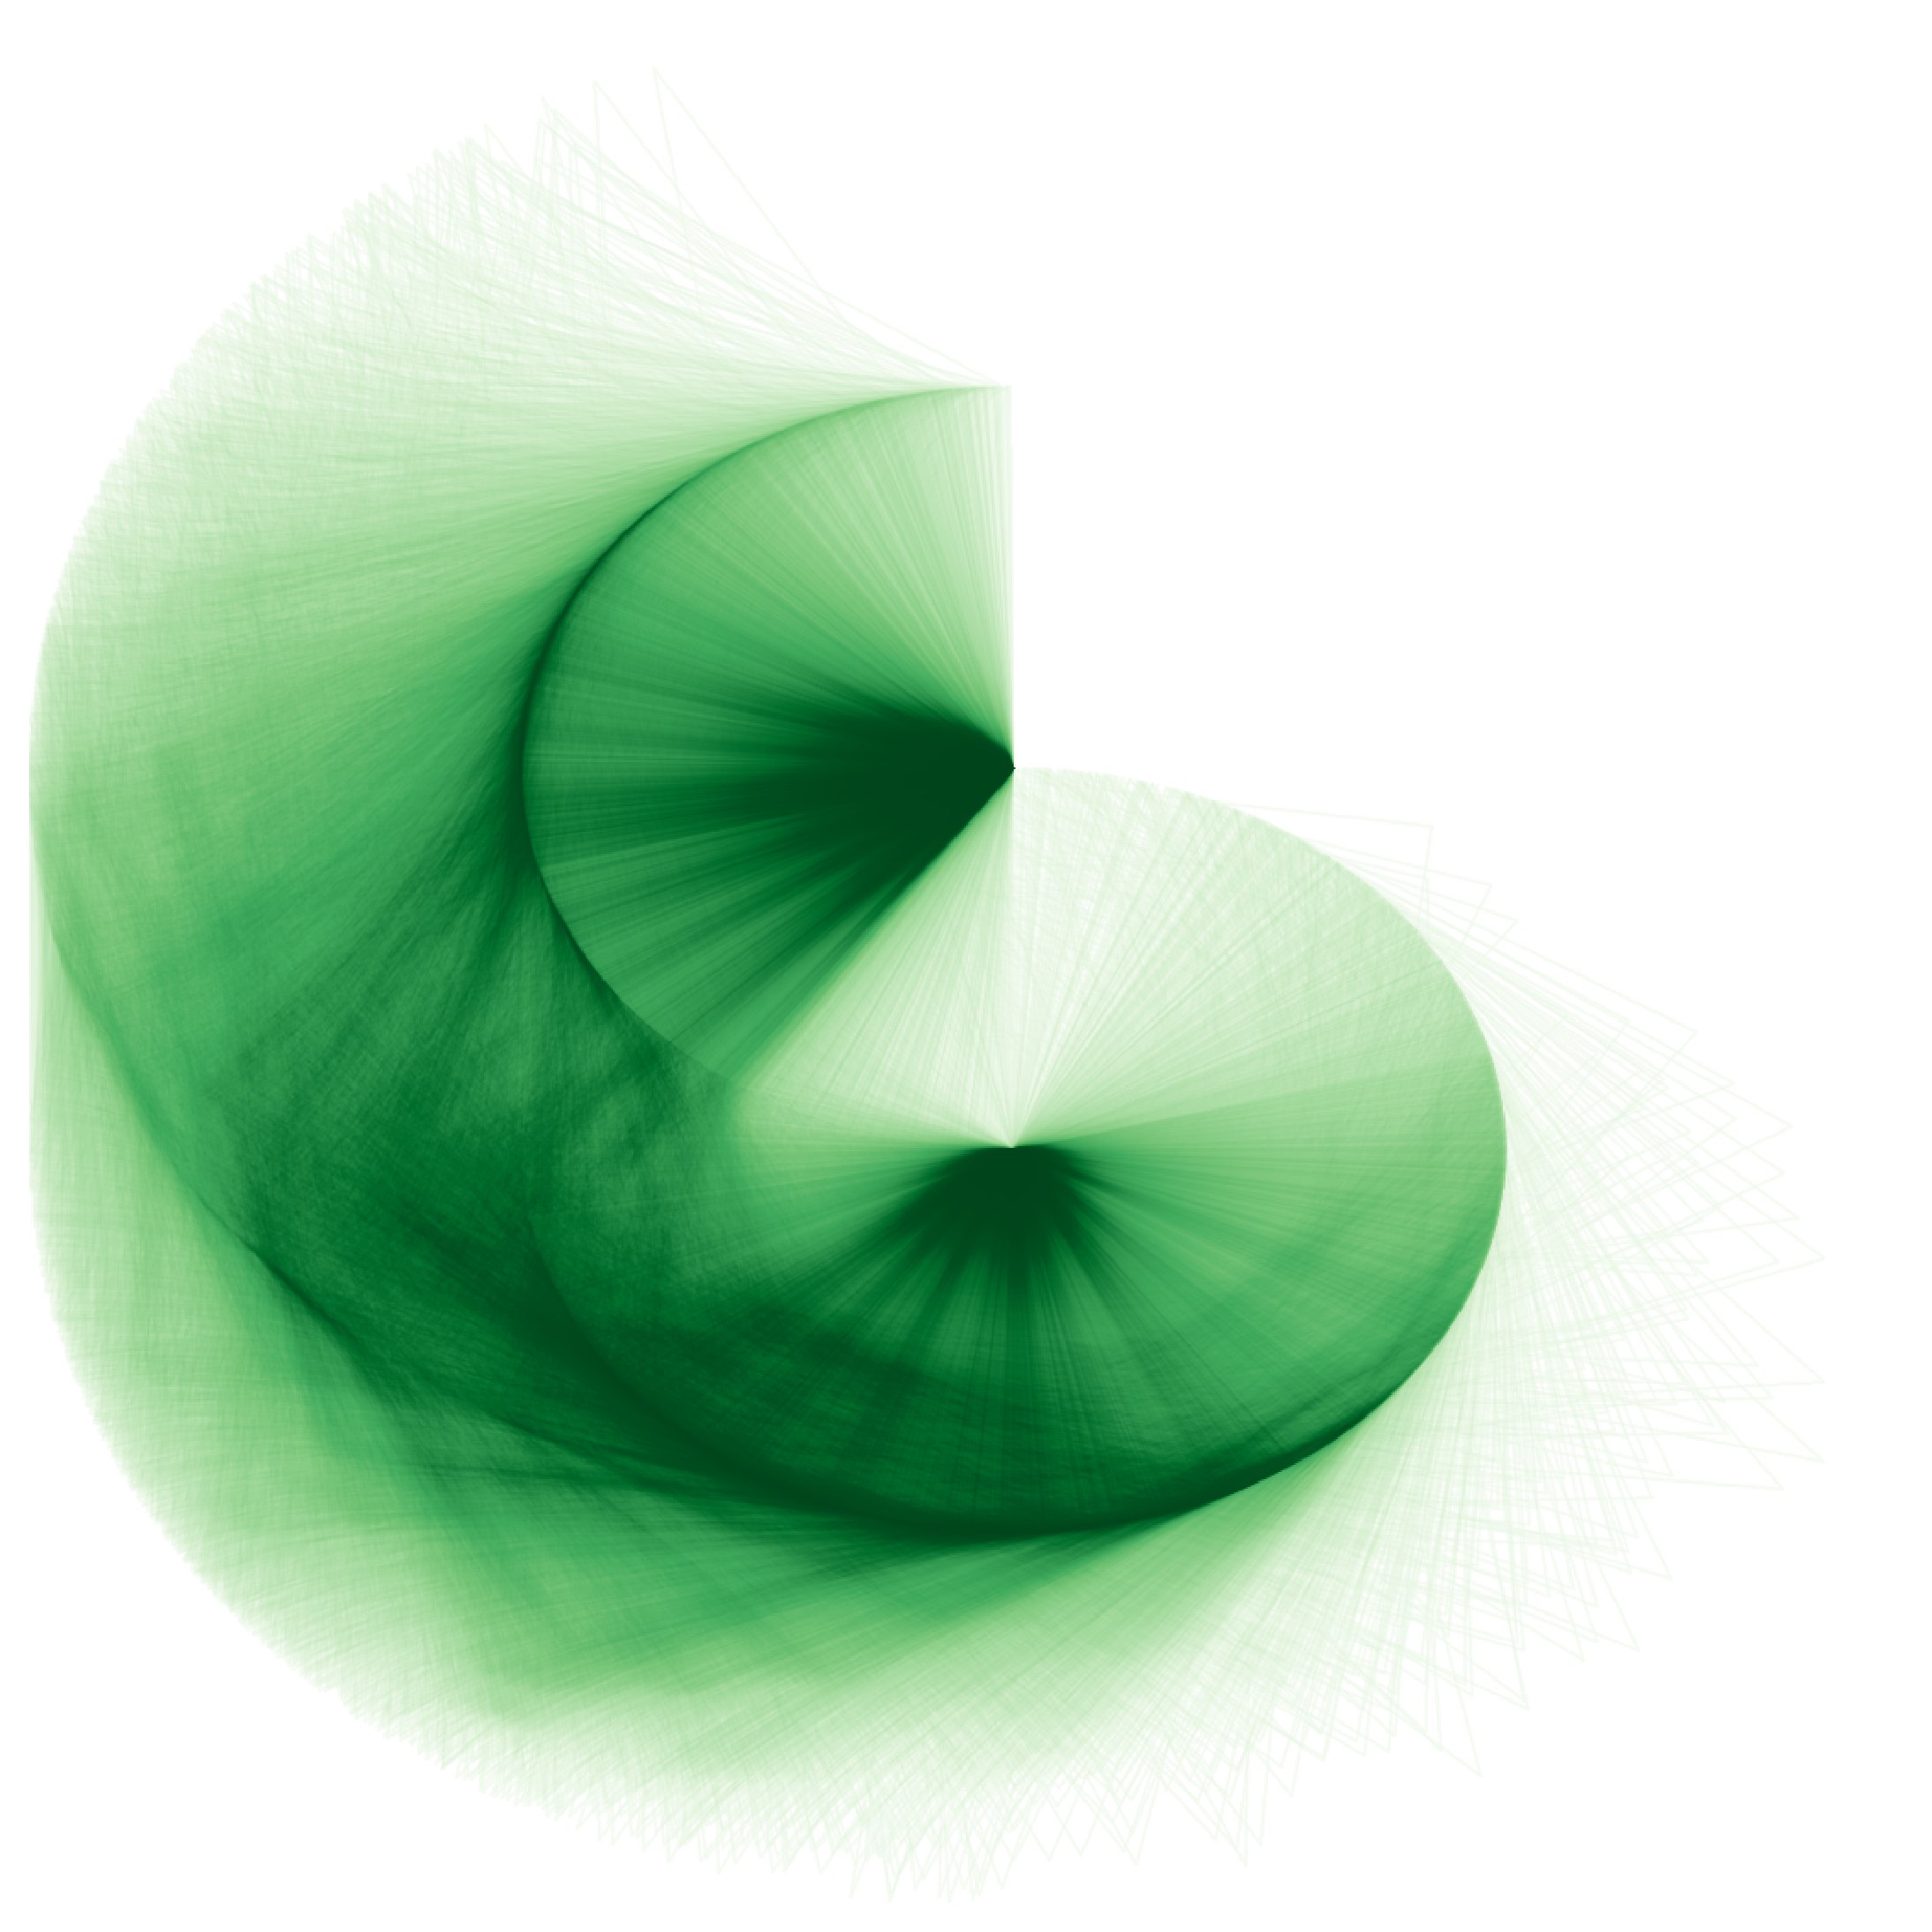
\includegraphics[width=\linewidth]{images/constraind_diffusion_rejection/loops_planar_reflected.pdf}
		\caption{Reflected samples.}
		\label{fig:loop_reflected}
	\end{subfigure}
	\hfill
	\begin{subfigure}[t]{0.23\textwidth}
		\centering
		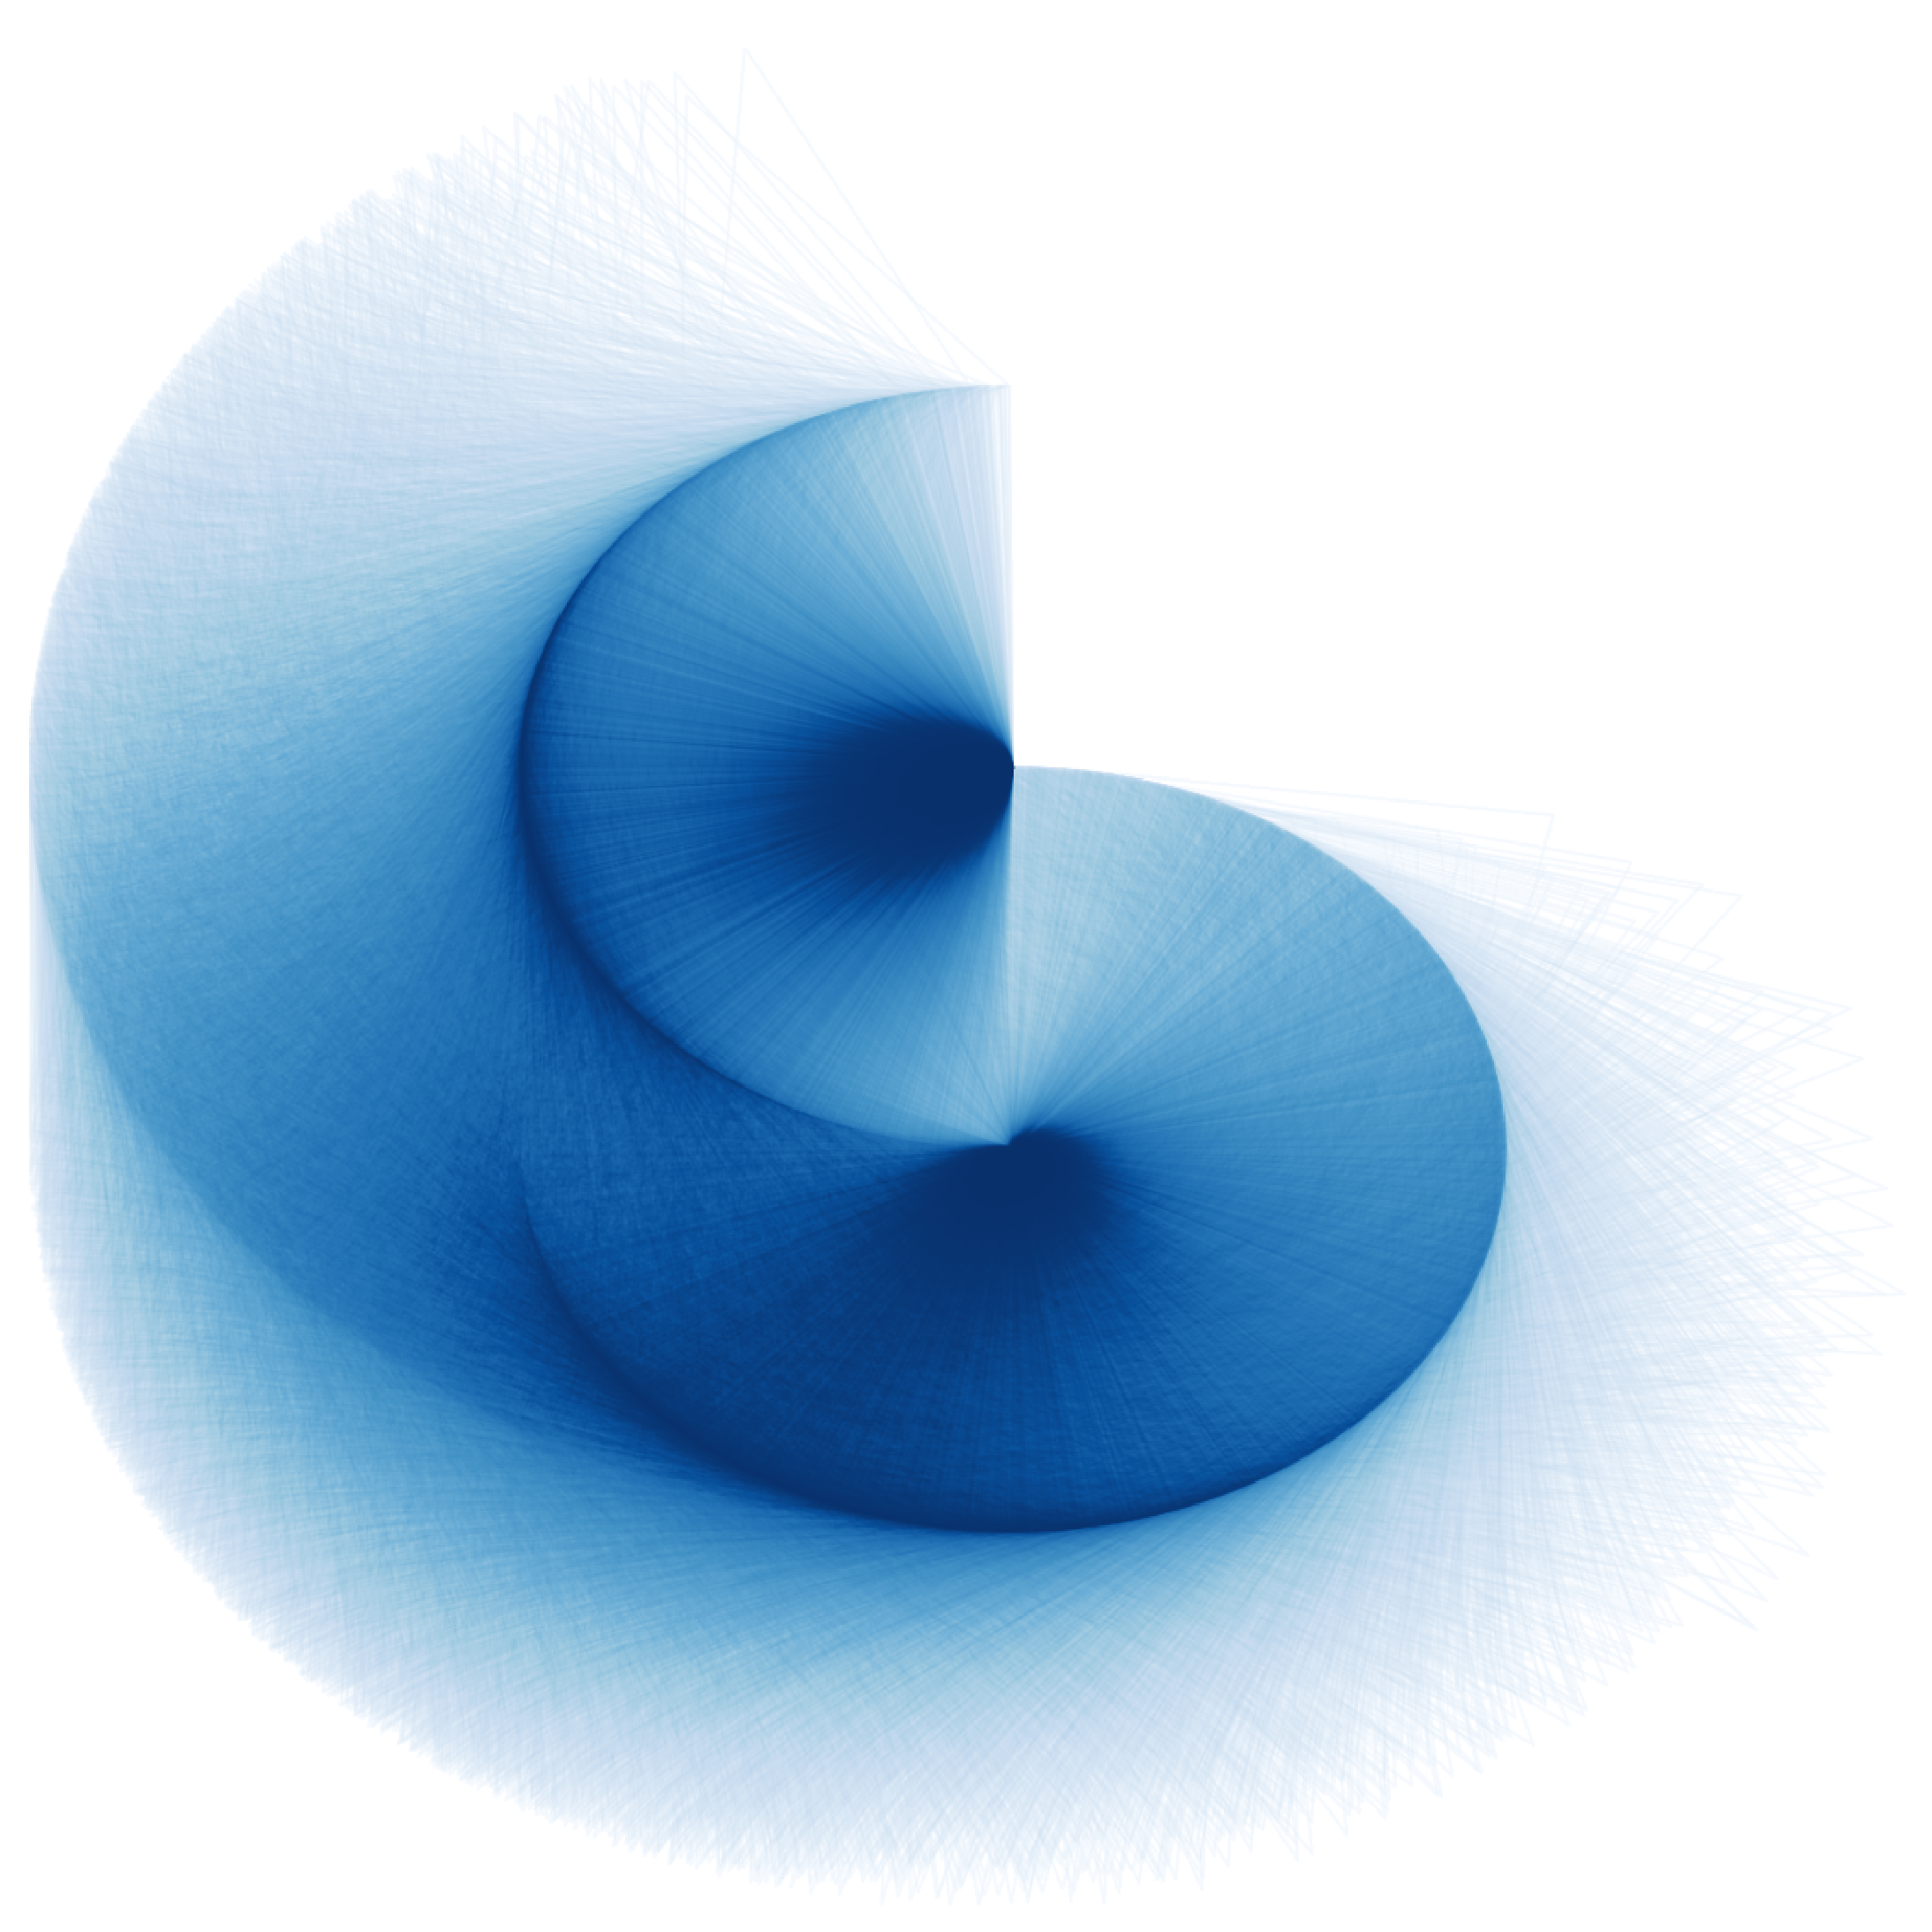
\includegraphics[width=\linewidth]{images/constraind_diffusion_rejection/loops_planar_uniform.pdf}
		\caption{Uniform distribution.}
		\label{fig:loop_uniform}
	\end{subfigure}
	\caption{A qualitative comparison of \(10^5\) samples from the data distribution,  our Metropolis diffusion model, a reflected diffusion model and the uniform distribution for the constrained conformational modelling of cyclic peptide backbones.
		For visual clarity, the figures only show the constrained planar projections encoded by \(\mathbb{P}\subset\R^3\).
	}
	\label{fig:loop}
\end{figure}

\begin{figure}[t]
	\centering
	\begin{subfigure}[t]{0.23\textwidth}
		\centering
		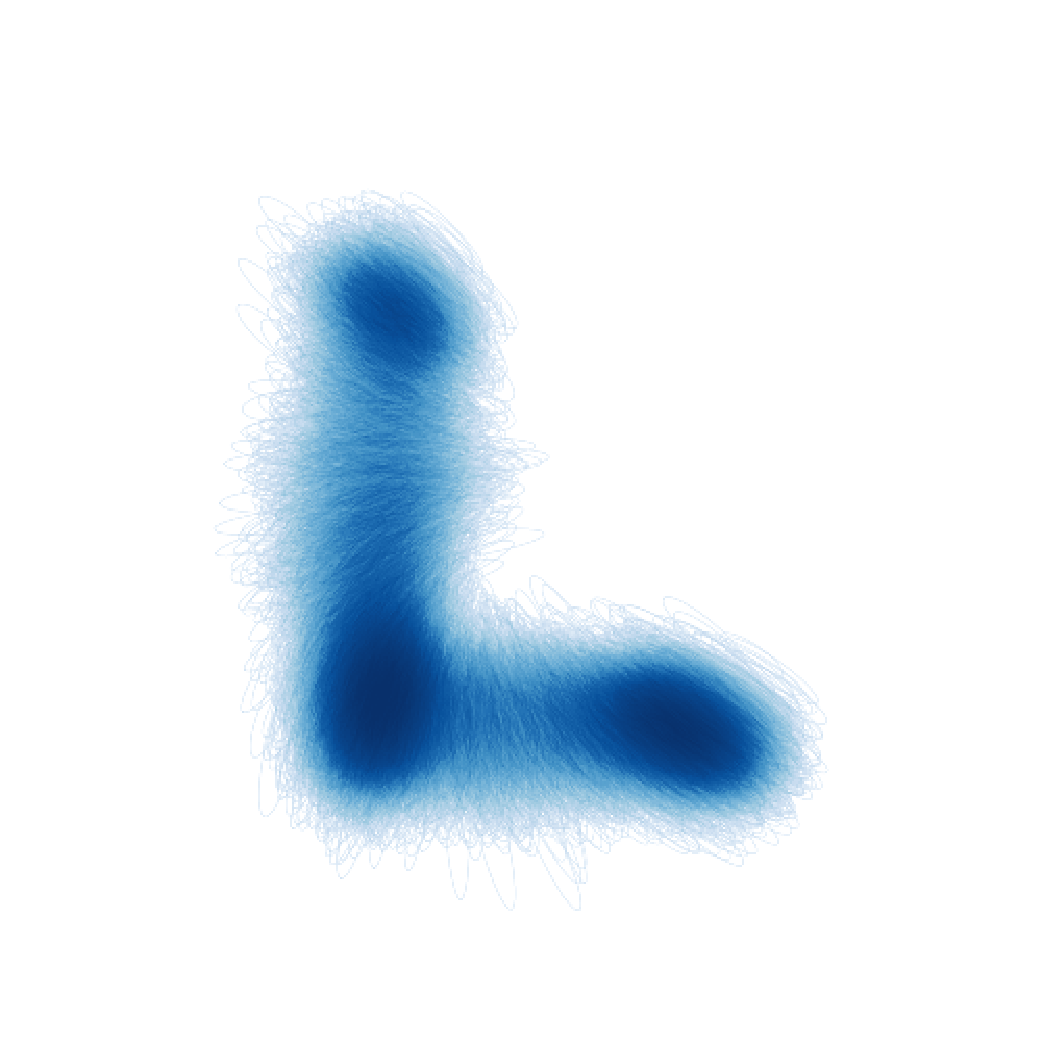
\includegraphics[width=\linewidth]{images/constraind_diffusion_rejection/spd_main_data.pdf}
		\caption{Data distribution.}
		\label{fig:loop_data}
	\end{subfigure}
	\hfill
	\begin{subfigure}[t]{0.23\textwidth}
		\centering
		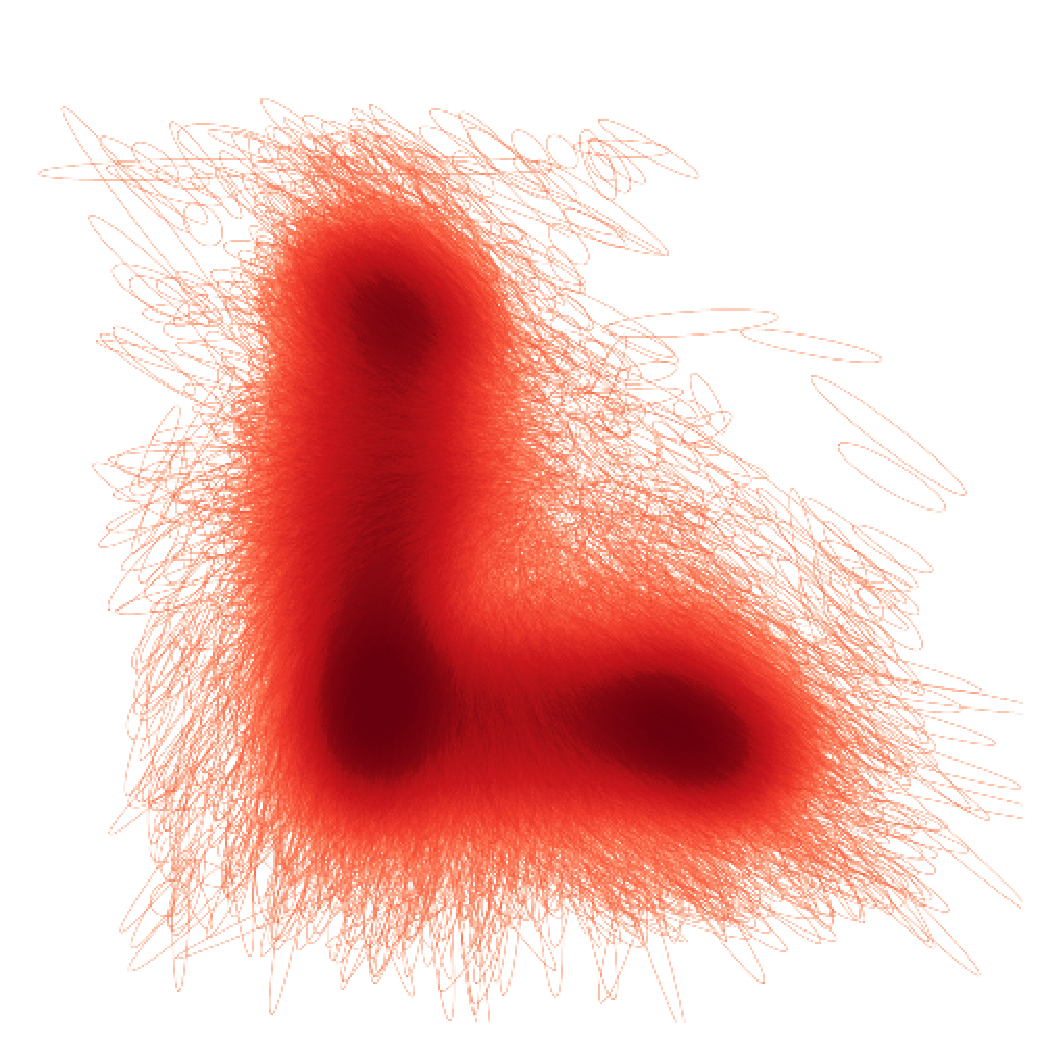
\includegraphics[width=\linewidth]{images/constraind_diffusion_rejection/spd_main_rejection.pdf}
		\caption{Metropolis samples.}
		\label{fig:loop_rejection}
	\end{subfigure}
	\hfill
	\begin{subfigure}[t]{0.23\textwidth}
		\centering
		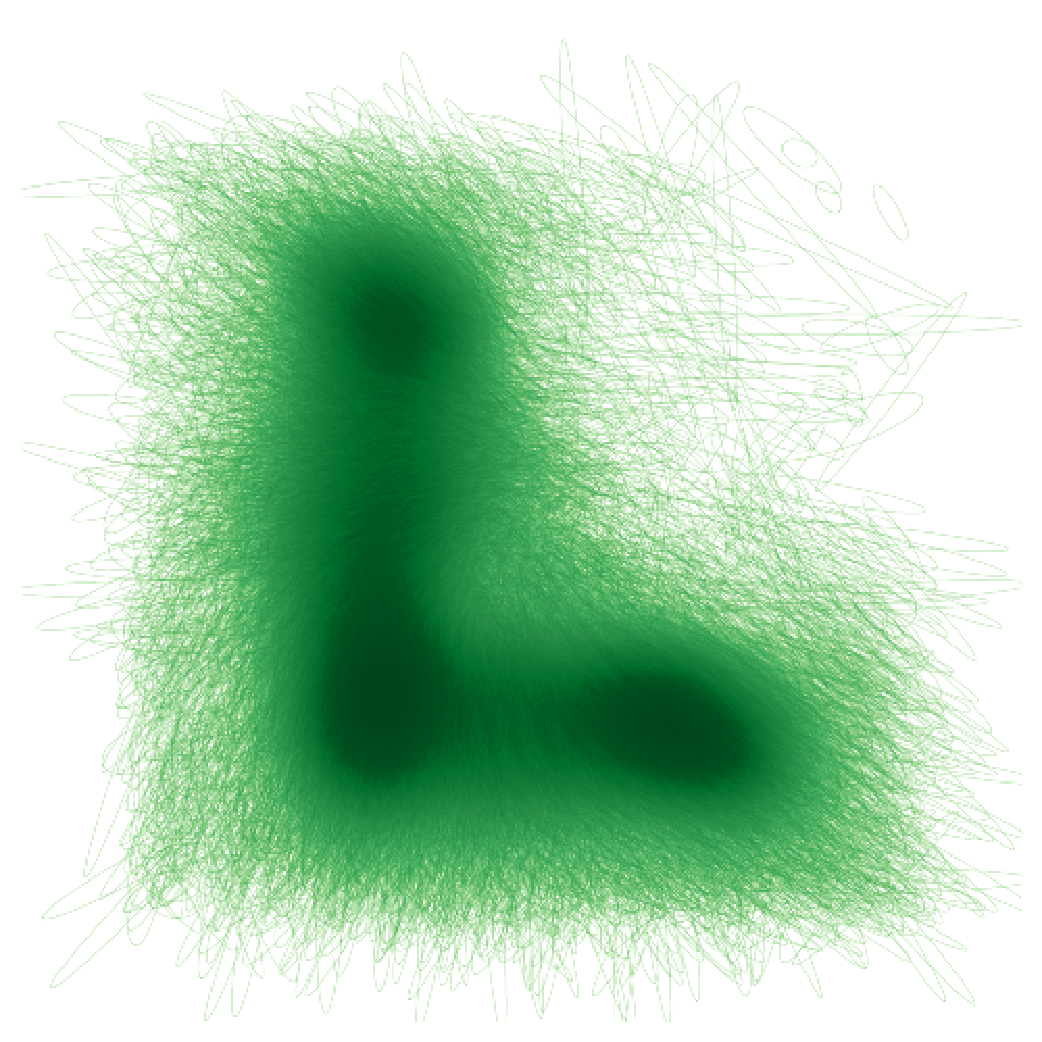
\includegraphics[width=\linewidth]{images/constraind_diffusion_rejection/spd_main_reflected.pdf}
		\caption{Reflected samples.}
		\label{fig:loop_reflected}
	\end{subfigure}
	\hfill
	\begin{subfigure}[t]{0.23\textwidth}
		\centering
		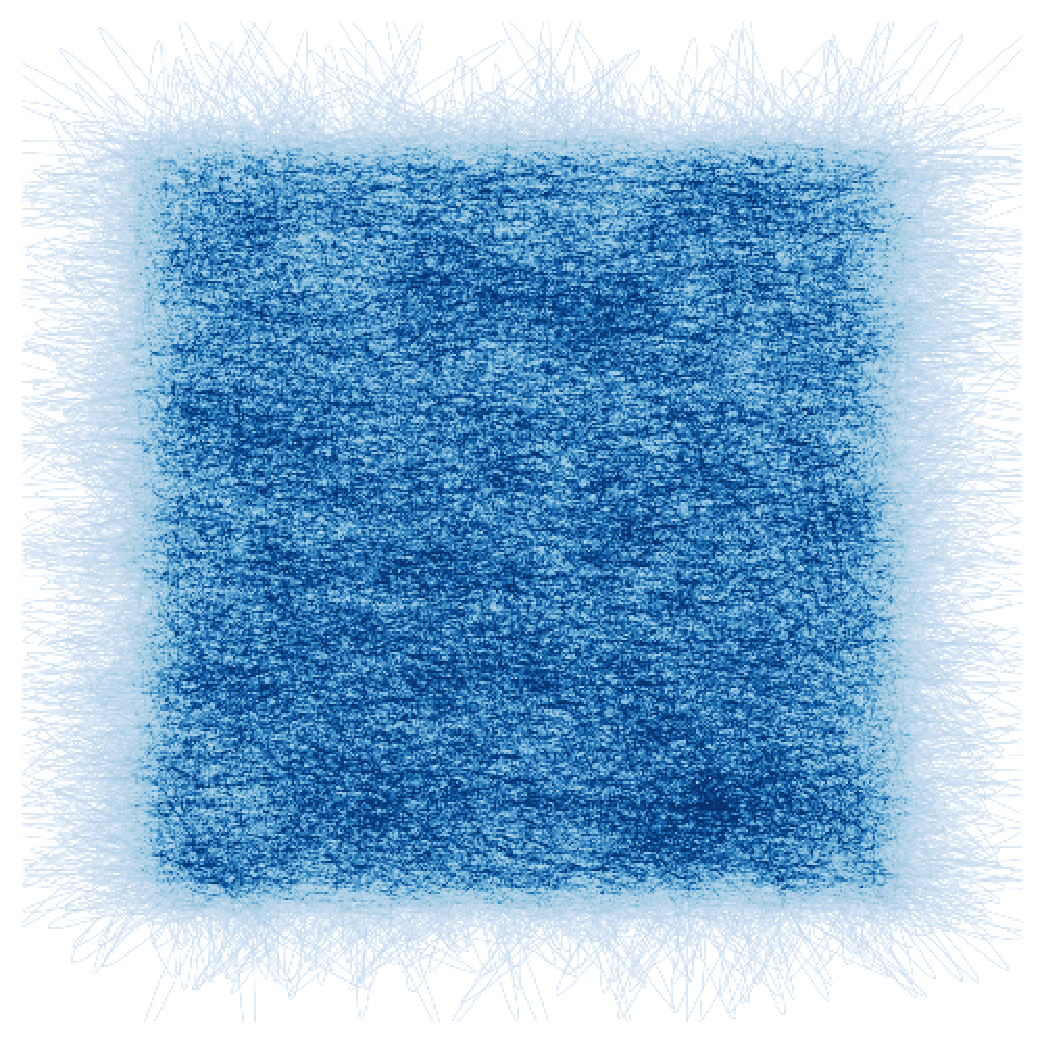
\includegraphics[width=\linewidth]{images/constraind_diffusion_rejection/spd_main_uniform.pdf}
		\caption{Uniform distribution.}
		\label{fig:loop_uniform}
	\end{subfigure}
	\caption{A qualitative comparison of \(10^5\) samples from the data distribution, our Metropolis diffusion model, a reflected diffusion model and the uniform distribution for the constrained modelling of manipulability ellipsoids of robotic arms.
		For visual clarity, the figures show the SPD matrices plotted.
	}
	\label{fig:robotic_arm}
\end{figure}

\begin{table}[h]
	\caption{
		Log-likelihood (\(\uparrow\)) of a held-out test set for the robotics and protein applications.
		Means and standard deviations are computed over 3 different runs.
		Training time in hours is listed in parentheses.
	}
	\label{tab:real_world_data}
	\centering
	\begin{tabular}{llll}
		\toprule
		\scshape Dataset  &\scshape Domain                                      & {\scshape Reflected \emph{(hours)}}     & {\scshape Metropolis \emph{(hours)}}             \\
		\midrule
		\scshape Robotics & \(\c{S}_{++}^2\times\R^2\)                  & \(8.39 \pm{.06}\) \emph{(9.52)}  & \(\mathbf{9.13 \pm{.03}}\) \emph{(1.36)}  \\
		\scshape Proteins & \(\mathbb{P}\subset\R^3\times\mathbb{T}^4\) & \(15.20\pm{.06}\) \emph{(24.80)} & \(\mathbf{15.33 \pm{.02}}\) \emph{(3.12)} \\
		\bottomrule
	\end{tabular}
\end{table}

\subsection{Modelling geospatial data within non-convex country borders}
\label{sec:exp_wildfires}

Motivated by the strong empirical performance of our approach on tasks with challenging convex constraints, we investigate its ability to approximate distributions whose support is restricted to manifolds with highly non-convex boundaries---a setting that is intractable with existing approaches.
To this end, we derived a geospatial dataset based on wildfire incidence rates within the continental United States and train a Metropolis diffusion model constrained by the corresponding country borders on the sphere \(\c{S}^2\).

\subsubsection{Dataset}
\label{sec:wildfire_data_dataset}
To create the dataset we retrieved the rasterised version of the wildfire data provided by \textcite{welty2020combined}.
This was converted it to a spherical geodetic coordinate system using the \textsc{Cartopy} library \parencite{Cartopy}, and drew a weighted subsample of size \num{1e6}.
We then retrieved the country borders of the continental United States from \textcite{natural_earth_data} and mapped them to the same geodetic reference frame as the wildfire data.
A visualization of the resulting dataset are presented in~\cref{fig:wildfire_data_dist}.

\subsubsection{Point-in-spherical-polytope algorithms}
\label{sec:wildfire_data_algo}

The support of the data-generating distribution we aim to approximate is restricted to a highly non-convex set on the sphere, \(\mathbb{P}\in\c{S}^2\), given by the country borders of the continental United States.
In order to apply our Metropolis method we need an efficient binary function to tell us if a point on the sphere lies inside this set.

To do so we adapt an efficient reformulation of the point-in-spherical-polygon algorithm \parencite{bevis1989locating} presented in \cite{ketzner2022robust}.
The algorithm requires the provision of a reference point \(r\in\c{S}^2\) known to be located in \(\mathbb{P}\) and determines whether \(q\) is inside or outside the polygon by checking whether the geodesic between \(r\) and \(q\) crosses the polygon an even or odd number of times.

Letting \(\Hat{x}\in\mathbb{R}^3\) denote the Cartesian coordinates of a point \(x\in\c{S}^2\) embedded in Euclidean space.
\cite{ketzner2022robust} rely on a Cartesian reference coordinate system \(\Hat{Q}\) (with its \(z\)-axis given by \(\Hat{r}\)) and the corresponding spherical coordinate system \(Q\) to decompose the edge-crossing condition of \textcite{bevis1989locating} into two efficiently computable parts.
That is, the geodesic between \(q\) and \(r\) crosses an edge \(e_i=(v_i, v_j)\) of the polygon if: \begin{enumerate}[label=(\roman*)] \item the longitude of \(q\) in \(Q\) is bounded by the longitudes of \(v_i\) and \(v_j\) in \(Q\), i.e. \[ \phi_{Q}(q)\in\cbr{\min\del{\phi_{Q}(v_i), \phi_{Q}(v_j)}, \max\del{\phi_{Q}(v_i), \phi_{Q}(v_j)}}, \] \item the plane specified by the normal vector \(\Hat{p}_i=\Hat{v}_i\times \Hat{v}_j\) represents an equator that separates \({q}\) and \({r}\) into two different hemispheres, i.e. $$ \operatorname{sign}(\langle \Hat{p}_i, \Hat{r} \rangle \cdot \langle \Hat{p}_i, \Hat{q} \rangle) = -1.
	      $$
\end{enumerate}

Especially when \(\mathbb{P}\) is fixed and the corresponding coordinate transformations and normal vectors can be precomputed for each edge, this algorithm affords an efficient and parallelisable approach to determining whether any given point on \(\c{S}^2\) is contained by a spherical polytope.

In order to discretise Brownian motion on the manifold we use modified geodesic random walks, \cref{sec:geodesic_random_walk}, by including the Metropolis step, \cref{alg:metropolis_approx}, to account for the reflection of the process.

\subsubsection{Results}

A qualitative visual comparison of samples from the true distribution, our model, and the uniform distribution is presented in~\cref{fig:wildfire_headline_plot} and a quantitative comparison to an unconstrained Riemannian score-based model from \cref{cpt:riemannian_score_based_models} is given in~\cref{tab:wildfire_riemann}.
This demonstrates that our approach is able to successfully model challenging multimodal and sparse distributions on non-flat constrained manifolds with highly non-convex boundaries.

\begin{table}[h]
    \setlength{\tabcolsep}{8pt}
    \caption{MMD ($\downarrow$) of a held-out test set for the geospatial modelling dataset. Means and standard deviations are computed over 3 different runs. Average training time is provided in hours.
    }
    \vspace{5pt}
    \label{tab:wildfire_riemann}
    \centering
    \begin{tabular}{ccccc}
    \toprule
    \scshape Model & \scshape Domain & \scshape MMD & \scshape runtime & \scshape {\% in boundary} \\
    \midrule 
     Unconstrained & $\mathcal{S}^2$ & $0.1567\pm_{0.013}$ & $\mathbf{0.81}$ & $63.3$\\
     Metropolis & $\mathbb{P}\subset\mathcal{S}^2$ & $\mathbf{0.1388\pm_{0.015}}$  & $3.86$ & $\mathbf{100.0}$\\
    \bottomrule
    \end{tabular}
\end{table}

\begin{figure}[t]
	\centering
	\begin{subfigure}[t]{0.28\textwidth}
		\centering
		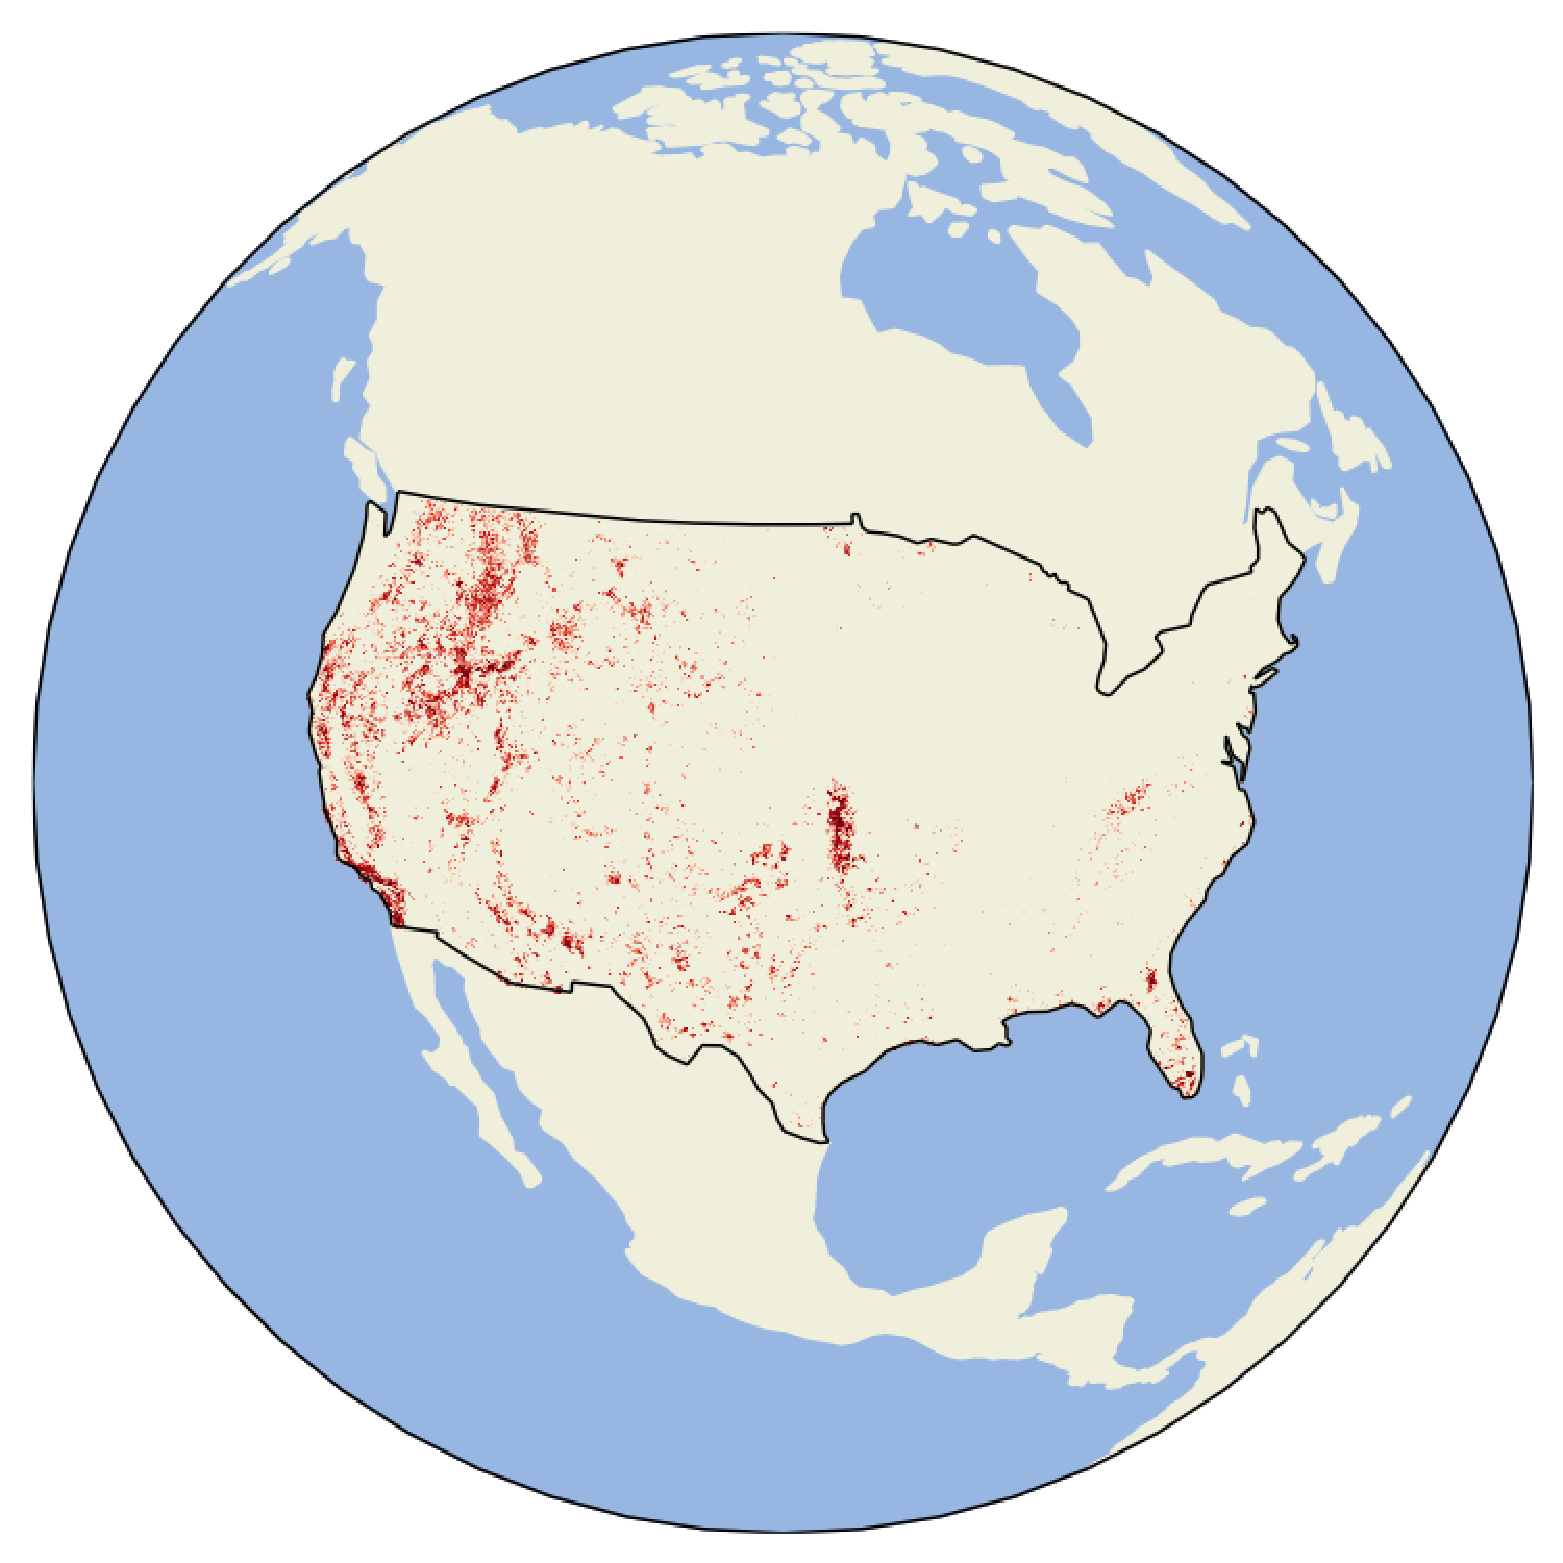
\includegraphics[width=\linewidth]{images/constraind_diffusion_rejection/wildfire_data_dist.pdf}
		\caption{Data distribution.}
		\label{fig:wildfire_data_dist}
	\end{subfigure}
	\hfill
	\begin{subfigure}[t]{0.28\textwidth}
		\centering
		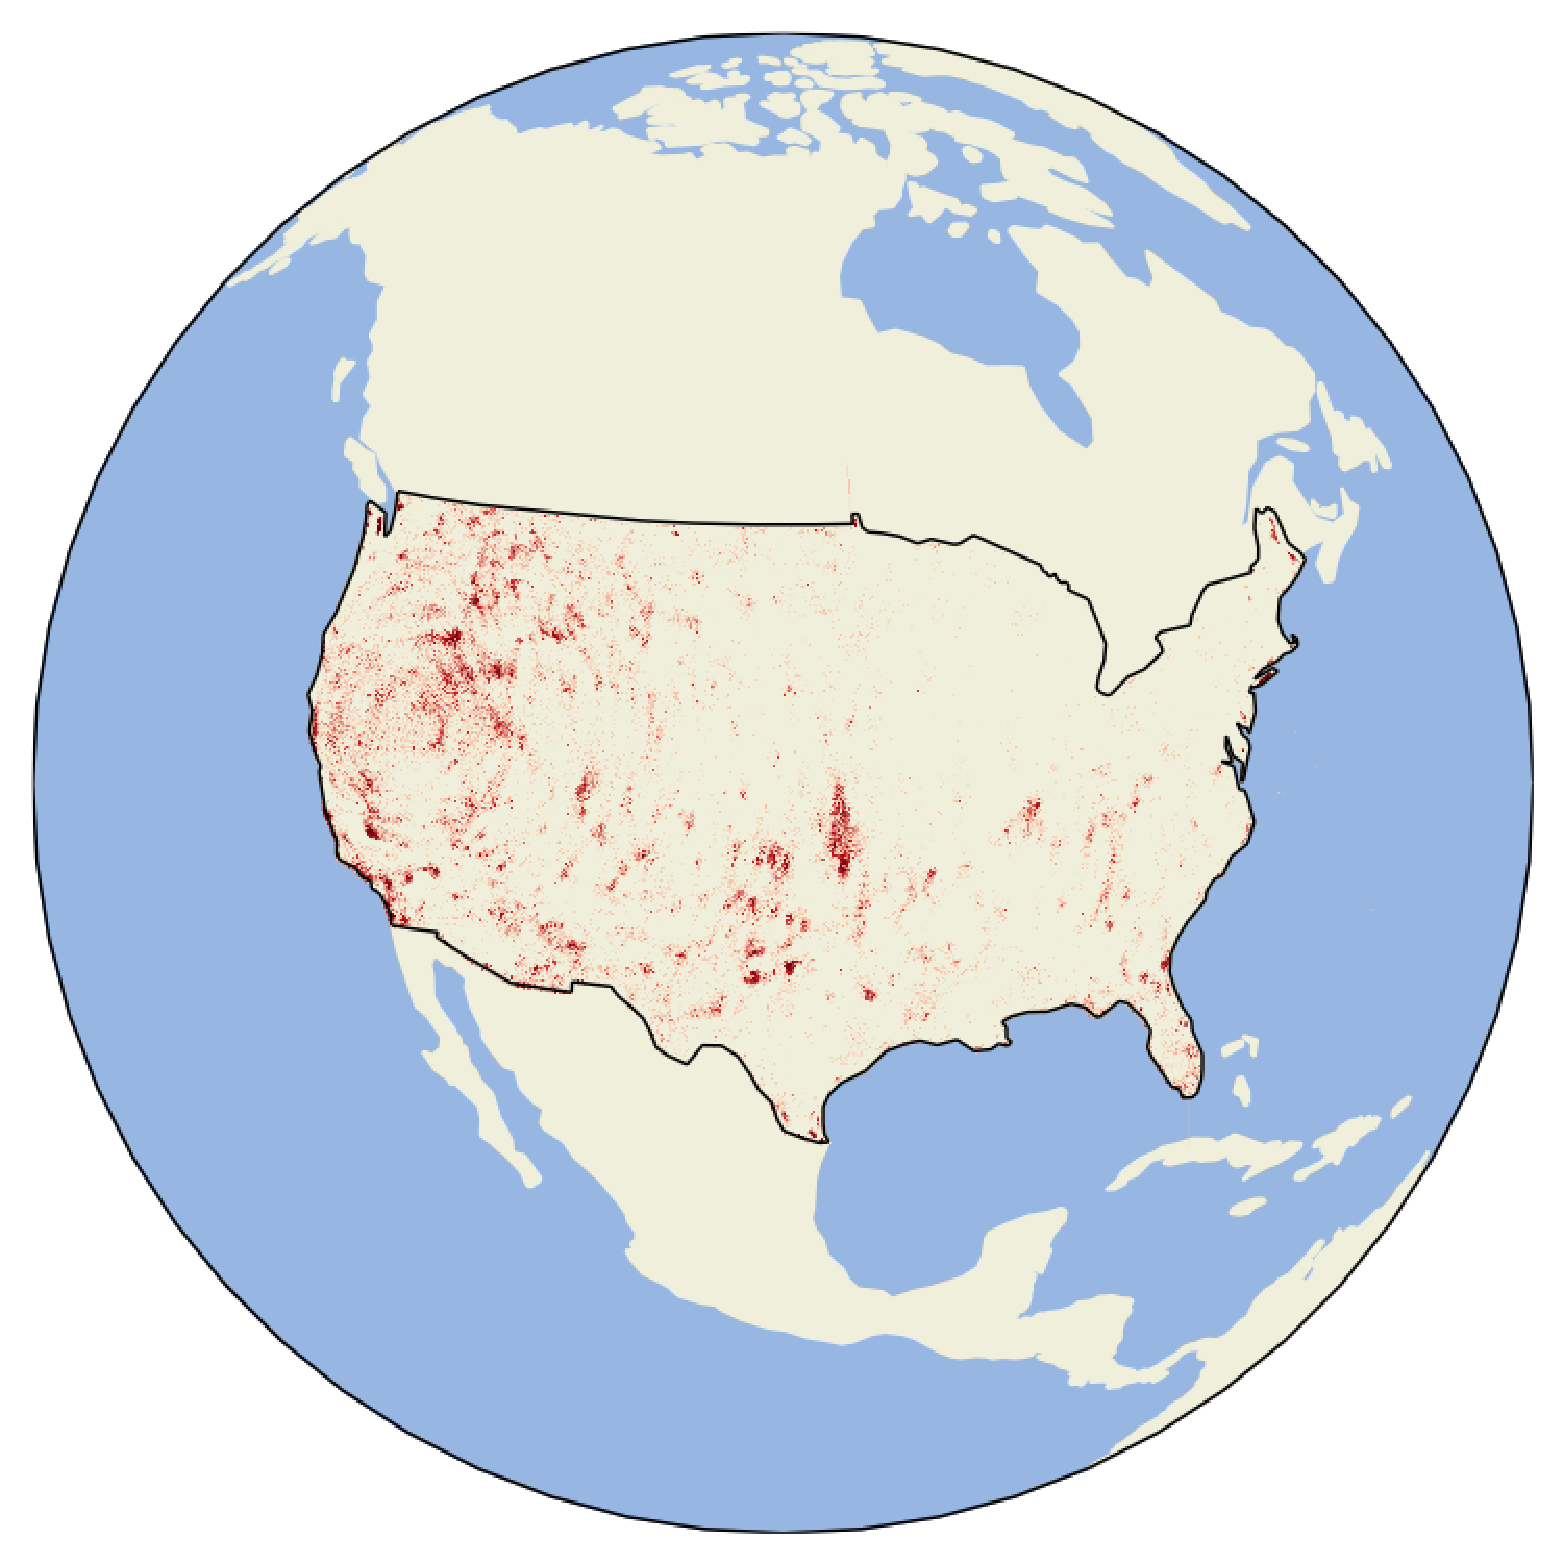
\includegraphics[width=\linewidth]{images/constraind_diffusion_rejection/wildfire_rejection_dist.pdf}
		\caption{Metropolis samples.}
		\label{fig:wildfire_rejection_dist}
	\end{subfigure}
	\hfill
	\begin{subfigure}[t]{0.28\textwidth}
		\centering
		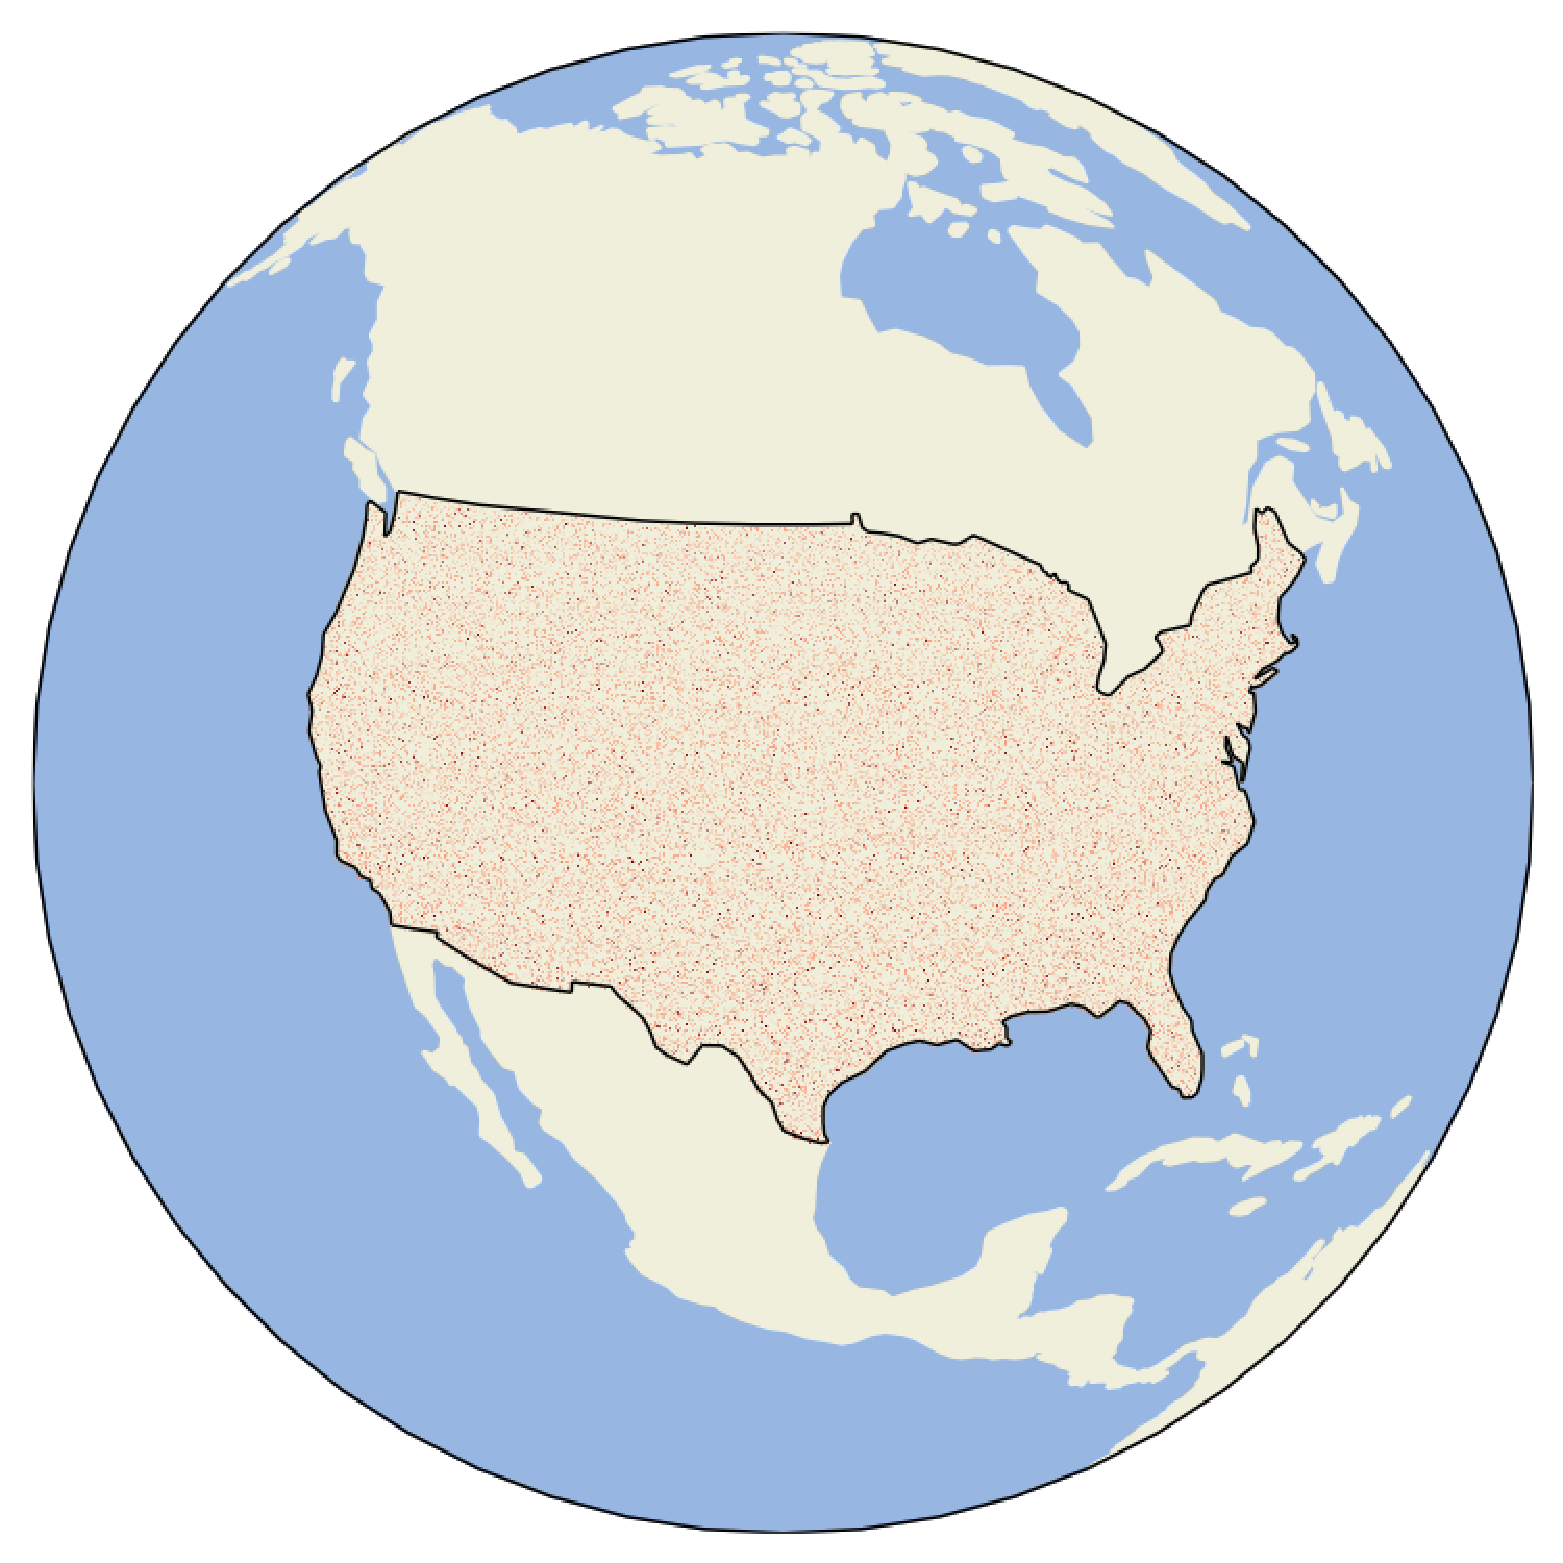
\includegraphics[width=\linewidth]{images/constraind_diffusion_rejection/wildfire_uniform_dist.pdf}
		\caption{Uniform distribution.}
		\label{fig:wildfire_uniform_dist}
	\end{subfigure}
	\caption{Orthographic projection of \(10^5\) samples from (a) the data distribution, (b) our Metropolis diffusion model, and (c) the uniform distribution, for geospatial data (wildfire incidence rates) within a non-convex boundary (the continental United States).
		The projections are aligned with the geometric centre of the boundary and zoomed in ten-fold for visual clarity.
	}
	\label{fig:wildfire_headline_plot}
\end{figure}

\section{Conclusion}

Accurately modelling distributions on constrained Riemannian manifolds is a challenging problem with a range of practical applications.
In this chapter, we have proposed a mathematically principled and computationally scalable extension of the existing diffusion model methodology to this setting.
Based on a \emph{Metropolisation} of random walks in Euclidean spaces and on Riemannian manifolds, we have shown that our approach corresponds to a valid discretisation of the reflected Brownian motion, justifying its use in diffusion models.
To demonstrate the practical utility of our method, we have performed an extensive empirical evaluation, showing that it outperforms existing constrained diffusion models on a range of synthetic and real-world tasks defined on manifolds with convex boundaries, including applications from robotics and protein design.
Leveraging the flexibility and simplicity of our method, we have also demonstrated that it extends beyond convex constraints and is able to successfully model distributions on manifolds with highly non-convex boundaries.

While we found our method to perform well across the synthetic and real-world applications we considered, we expect it to perform poorly on certain constraint geometries.
For instance, the current implementation relies on an isotropic noise distribution which could impede its performance on exceedingly narrow constraint geometries, even with correspondingly small step sizes.
In this context, an important direction of future research would be to investigate whether we can instead sample from more suitable distributions, e.g. a Dikin ellipsoid, while maintaining the simplicity and efficiency of the Metropolis approach.
More general topics of future work include the derivation of quantitative weak and mean square errors of our proposed discretisation scheme, as well as its application to more semantic constraints, for example with the objective of imposing sparsity in a basis or fixing the colour or style of an image.
